\documentclass[journal]{IEEEtran}
\usepackage[a5paper, margin=10mm]{geometry}
%\usepackage{lmodern} % Ensure lmodern is loaded for pdflatex
\usepackage{tfrupee} % Include tfrupee package


\setlength{\headheight}{1cm} % Set the height of the header box
\setlength{\headsep}{0mm}     % Set the distance between the header box and the top of the text


%\usepackage[a5paper, top=10mm, bottom=10mm, left=10mm, right=10mm]{geometry}

%
\usepackage{gvv-book}
\usepackage{gvv}
%\setlength{\intextsep}{10pt} % Space between text and floats

\makeindex

\begin{document}
\bibliographystyle{IEEEtran}
\onecolumn


\title{
	%\begin{flushleft}
	\begin{center}
	%MATRICES \\ In Geometry
	Discrete Mathematics
	\\
\rule{0.4\columnwidth}{0.4pt}
%\end{flushleft}
\end{center}
}
\author{
\vspace{11cm}
	%\begin{flushleft}
	\begin{center}
\includegraphics[width=0.2\columnwidth]{figs/logo.jpg}
\\
		{\huge	G. V. V. Sharma}\\Associate Professor,\\Department of Electrical Engineering, \\ IIT Hyderabad
	\end{center}
	%\end{flushleft}
%\IEEEpubid{\makebox[\columnwidth]{978-1-7281-5966-1/20/\$31.00 ©2020 IEEE \hfill} \hspace{\columnsep}\makebox[\columnwidth]{ }}
}
\maketitle

\newpage
\section*{About this Book}

This book introduces progressions, binomial theorem, limits and sequences. 
 All problems in the book are from NCERT mathematics textbooks from Class 9-12.  Exercises are from CBSE, JEE and Olympiad exam papers.   

There is no copyright, so readers are free to print and share.  

%This book is dedicated to my Hindi teacher in school, Shri Mandavi.
\begin{flushright}
\today
\end{flushright}
Github: https://github.com/gadepall/algebra
		\\
License: https://creativecommons.org/licenses/by-sa/3.0/
\\
and
\\
https://www.gnu.org/licenses/fdl-1.3.en.html

\newpage


\tableofcontents

\newpage
%\twocolumn
\onecolumn


%\renewcommand{\theequation}{\theenumi}
\numberwithin{equation}{enumi}
%\numberwithin{figure}{enumi}
\numberwithin{figure}{subsection}
%\renewcommand{\thefigure}{\theenumi}
\renewcommand{\thetable}{\theenumi}

\section{Arithmetic Progression}
\subsection{Formulae}
\begin{enumerate}[label=\thesubsection.\arabic*,ref=\thesubsection.\theenumi]
	\item Find the sum
\begin{align}
	\label{eq:ap-sum10}
	S = 1 + 2 + \dots + 10
\end{align}
\solution Reversing the sum in
	\eqref{eq:ap-sum10}
	as
\begin{align}
	\label{eq:ap-sum10-rev}
	S = 10 + 9 + \dots + 1
\end{align}
and adding 
	\eqref{eq:ap-sum10}
	and
	\eqref{eq:ap-sum10-rev},
\begin{align}
	\label{eq:ap-sum10-add}
	2S &= 11 + 11 + \dots + 11 \quad 10 \text{ times}
	\\
	\implies S &= \frac{11 \times 10}{2} = 55
\end{align}
\item The sum of the first $n$ natural numbers is
\begin{align}
	\sum_{k=1}^{n}k &= 1+ 2 + \dots + n
	\\
	&= \frac{n\brak{n+1}}{2}
	\label{eq:ap-sumn}
\end{align}
\item The $n^{th}$ term of an arithmetic progression (AP) is
\begin{align}
	\label{eq:ap-nthterm}
	x(n) = x(0) + nd, \quad n = 0, 1, \dots
\end{align}
\item 
\begin{align}
	\label{eq:ap-nsum}
	 y(n)=\sum_{k=0}^{n}x(k) = \frac{n+1}{2}\brak{x(0) + \frac{dn}{2}}
\end{align}
\solution
From
	\eqref{eq:ap-nthterm}
	and
	\eqref{eq:ap-nsum},
\begin{align}
	\label{eq:ap-nthsum}
	 \sum_{k=0}^{n}x(k) &= 
\sum_{k=0}^{n}
	 \brak{x(0) + kd} 
	 \\
	 &= 
\sum_{k=0}^{n}x(0) + 
d\sum_{k=1}^{n}k
	  = \brak{n+1}x(0) + d\frac{n\brak{n+1}}{2}
\end{align}
upon substituting from
	\eqref{eq:ap-sumn}, yielding
	\eqref{eq:ap-nthsum}
	upon simplification.
\end{enumerate}

\subsection{NCERT}
\begin{enumerate}[label=\thesubsection.\arabic*, ref=\thesubsection.\theenumi]
\item Determine the AP whose 3rd term is 5 and the 7th term is 9.
	\\
	\solution
\begin{align}
	a_0+n_1d &= a_2
	\\
	a_0+n_2d &= a_6
	\\
	\implies 
	\myvec{
	1&n_1 
	\\
	1&n_2 
}
	\myvec{
a_0
\\
	d}
	\myvec{
a_2
\\
	a_6}
       \end{align}
Substituting numerical values 
yields
\begin{align}
	\myvec{1 & 2 \\ 1 & 6}
	\myvec{a_0 \\ d}
	&=
	\myvec{5\\9}
	\\
	\implies \myvec{a_0 \\ d}
	&=
	\myvec{3\\1}
\end{align}
%
\item For the AP 
$$\frac{3}{2}, \frac{1}{2}, -\frac{1}{2}, -\frac{3}{2}, \dots $$ write the first term $a_0$ and the common difference $d$.
\\
\solution
\begin{align}
	a_0 = \frac{3}{2}, d=  \frac{1}{2}-\frac{3}{2} = -1.
\end{align}
\item Which of the following list of numbers form an AP? If they form an AP, 
write the next two terms 
		\begin{multicols}{2}
\begin{enumerate}
\item $4, 10, 16, 22, \dots$ 
\item $-2, 2, -2, 2, -2, \dots$
\item $1, -1, -3, -5, \dots$ 
\item $1, 1, 1, 2, 2, 2, 3, 3, 3, \dots$
\end{enumerate}
\end{multicols}
\begin{enumerate}
	\item AP
\begin{align}
	a_0 &= 4, d = 6
	\\
	\implies a_n &= 4 +6n
	\\
	\text{or, }a_4 = 28, a_5 = 34.
\end{align}
	\item 
		Not an AP.
\begin{align}
	 a_1-a_0=4
	\\
	 a_2-a_1=-4
\end{align}
\end{enumerate}
\item Find the 10th term of the AP : $2,  7,  12,  \dots$
\item Which term of the AP : $21,  18,  15,  \dots$ is - 81? Also,  is any term 0? Give reason for your answer.
	\\
	\solution
\begin{align}
	a_0 &= 21, d = -6
	\\
	\implies a_n &= 21 -6n
	\label{eq:ap-21}
	\\
	\text{or, }-81 &=21-6n \implies n = 17
\end{align}
If
\begin{align}
	a_n = 0, 
 n= \frac{21}{6}
\end{align}
	using \eqref{eq:ap-21} which is impossible.
\item Check whether 301 is a term of the list of numbers $5,  11,  17,  23,  \dots$
\item How many two-digit numbers are divisible by 3?
\item Find the 11th term from the last term (towards the first term) of the
AP : $10,  7,  4,  \dots,  - 62$.
	\\
	\solution Reversing the AP,
\begin{align}
	a_0 &= -62, d = 3, 
	\\
	\implies a_{10}&=-62+10\times 3 = -32
\end{align}
upon substituting in
	\eqref{eq:ap-nthterm}.
\item A sum of \rupee 1000 is invested at $8\%$ simple interest per year. Calculate the interest at the end of each year. Do these interests form an AP? If so,  find the interest at the end of 30 years making use of this fact.
\item In a flower bed,  there are 23 rose plants in the first row,  21 in the
second,  19 in the third,  and so on. There are 5 rose plants in the last row. How many rows are there in the flower bed?
\item Find the sum of the first 22 terms of the AP : $8,  3,  -2,  \dots$
	\\
	\solution
\begin{align}
a_0 = 8, d = -5, n = 21
\\
\implies 
	S_{21} = -979
\end{align}
upon substituting in 
	\eqref{eq:ap-nsum}.
\item If the sum of the first 14 terms of an AP is 1050 and its first term is 10,  find the 20th term.
	\\
	\solution
	\begin{align}
		S_{13} &= 1050, a_0 = 10, n = 13
		\\
		\implies 1050 &= 14\brak{10+\frac{13d}{2}}
		\\
		\text{or, } d&= 10
		\\
		\therefore
		a_{19} &= 10+19d = 200
	\end{align}
\item How many terms of the AP : $24,  21,  18,  \dots$ must be taken so that their
sum is 78?
\item Find the sum of 
\begin{enumerate}
\item the first 1000 positive integers.
\item the first $n$ positive integers.
\end{enumerate}
\item Find the sum of first 24 terms of the list of numbers whose $n^{th}$ term is given by $a_n = 3 + 2n$
	\\
	\solution
\begin{align}
	\sum_{k=1}^{n}a_k &= \sum_{k=1}^{n}3 + \sum_{k=1}^{n}2k
	\\
	&=3n + 2\frac{n\brak{n+1}}{2} = n\brak{n+4}
	\\
	&= 672
\end{align}
upon substituting numerical values.
\item A manufacturer of TV sets produced 600 sets in the third year and 700
sets in the seventh year. Assuming that the production increases uniformly by a fixed number every year,  find 
\begin{enumerate}
\item   the production in the 1st year
\item	the production in the 10th year
\item the total production in first 7 years.
\end{enumerate}
\item In which of the following situations,  does the list of numbers involved make an arithmetic progression,  and why?
\begin{enumerate}
\item The taxi fare after each km when the fare is \rupee 15 for the first km and \rupee 8 for each additional km.
\item The amount of air present in a cylinder when a vacuum pump removes 
$\frac{1}{4}$ of the air remaining in the cylinder at a time.
\item  The cost of digging a well after every metre of digging,  when it costs \rupee 150 for the first metre and rises by \rupee 50 for each subsequent metre.
\item The amount of money in the account every year,  when \rupee 10000 is deposited at compound interest at 8 \% per annum.
\end{enumerate}
\item Write first four terms of the AP,  when the first term $a$ and the common difference $d$ are
given as follows
		\begin{multicols}{2}
\begin{enumerate}
\item $a = 10,  d = 10	$	
\item $a = 4,  d = -3	$	
\item $a = -2,  d = 0	$	
\item $ a = -1,  d =\frac{1}{2}$
\item $a = -1.25,  d = -0.25$	
\end{enumerate}
\end{multicols}
\item For the following APs,  write the first term and the common difference
	\begin{multicols}{2}
		\begin{enumerate}[itemsep=1ex]
\item $3,  1,  -1,  -3,  \dots $
\item $-5,  -1,  3,  7,  \dots $
\item $\frac{1}{3},  \frac{5}{3},  \frac{9}{3},  \frac{13}{3}, \dots $
\item $0.6,  1.7,  2.8,  3.9, \dots $ 
\end{enumerate}
\end{multicols}
\item Which of the following are APs? If they form an AP,  find the common difference $d$ and
write three more terms.
\begin{multicols}{2}
\begin{enumerate}[itemsep=1ex]
\item $2,  4,  8,  16,  \dots $
\item $2, \frac{5}{2},  3,  \frac{7}{2}, \dots $
\item $-1.2,  -3.2,  -5.2,  -7.2,  \dots $
\item $-10,  -6,  -2,  2,  \dots $
\item $3, 3+\sqrt{2},  3+2\sqrt{2},  3+3\sqrt{2}, \dots $
\item $0.2,  0.22,  0.222,  0.2222,  \dots $
\item $0,  -4,  -8,  -12,  \dots $
\item $-\frac{1}{2},  -\frac{1}{2},  -\frac{1}{2},  -\frac{1}{2}, \dots $
\item $1,  3,  9,  27, \dots $ 
\item $a,  2a,  3a,  4a, \dots $ 
\item $a,  a^2,  a^3,  a^4, \dots $
\item $\sqrt{2},  \sqrt{8},  \sqrt{18},  \sqrt{32}, \dots $
\item $\sqrt{3},  \sqrt{6},  \sqrt{9},  \sqrt{12}, \dots $
\item $1^2,  3^2,  5^2,  7^2, \dots$
\item $1^2,  5^2,  7^2,  73, \dots $
\end{enumerate}
\end{multicols}
\item Fill in the blanks in 
	\tabref{table:ap},  given that $a$ is the first term,  $d$ the common
difference and $a_n$ the $n^{th}$ term of the AP.
\begin{table}[H]
	\centering
\begin{tabular}{|c|c|r|l|l|}
\hline
\\
&$a$& $d$ & $n$ & $a_n$
\\
\hline
(i)& 	7 &3 &8 &$\dots $ 
\\
(ii)& 	-18 &$\dots $  &10  &0
\\
(iii)& 	$\dots $  &-3 &18 &-5
\\
(iv)& 	-18.9 &2.5 &$\dots $  &3.6
\\
(v)& 	3.5 &0 &105 &$\dots $ 
\\
\hline
\end{tabular}
	\caption{}
	\label{table:ap}
\end{table}
\item Choose the correct choice in the following and justify 
\begin{enumerate}
	\item $30^{th}$ term of the AP: $10,  7,  4, \dots $   is
	\begin{multicols}{4}
\begin{enumerate}
\item 97
\item 77
\item -77
\item -87
\end{enumerate}
\end{multicols}
\item $11^{th}$ term of the AP: $ -3,  -\frac{1}{2},  2, \dots  $ is 
	\begin{multicols}{4}
\begin{enumerate}
\item 28
\item 22
\item -38
\item $-48\frac{1}{2}$
\end{enumerate}
\end{multicols}
\item In the following APs,  find the missing terms in the blanks  
	\begin{multicols}{2}
\begin{enumerate}
\item $2,  \dots,  26$
\item $\dots  ,  13, \dots  ,  3$
\item $5,  \dots  ,  \dots  ,  9\frac{1}{2}$
\item $-4,  \dots  ,  \dots  ,  \dots  ,  \dots,  6$
\item $\dots ,  38,  \dots ,  \dots ,  \dots ,  -22$
\end{enumerate}
\end{multicols}
\end{enumerate}
\item Which term of the AP : $3,  8,  13,  18,  \dots $ is 78?
\item Find the number of terms in each of the following APs:
\begin{enumerate}
	\item $7,  13,  19,  \dots , 205$.
	\item $18,  15\frac{1}{2},  13, \dots , -47$
\end{enumerate}
\item Check whether -150 is a term of the AP : $11,  8,  5,  2 \dots $ 
\item Find the 31st term of an AP whose 11th term is 38 and the 16th term is 73.
\item An AP consists of 50 terms of which 3rd term is 12 and the last term is 106. Find the 29th term.
\item If the 3rd and the 9th terms of an AP are 4 and -8 respectively,  which term of this AP is zero?
\item The 17th term of an AP exceeds its 10th term by 7. Find the common difference.
\item Which term of the AP : $3,  15,  27,  39, \dots $  will be 132 more than its 54th term? 
\item How many three-digit numbers are divisible by 7?
\item How many multiples of 4 lie between 10 and 250?
\item For what value of $n$,  are the $n^{th}$ terms of two APs: $63,  65,  67, \dots $  and $3,  10,  17, \dots $  equal?
\item Determine the AP whose third term is 16 and the 7th term exceeds the 5th term by 12.
\item Find the 20th term from the last term of the AP : $3,  8,  13, \dots  ,  253$.
\item The sum of the 4th and 8th terms of an AP is 24 and the sum of the 6th and 10th terms is 44. Find the first three terms of the AP.
\item Subba Rao started work in 1995 at an annual salary of \rupee 5000 and received an increment of \rupee 200 each year. In which year did his income reach \rupee 7000?
\item Ramkali saved \rupee 5 in the first week of a year and then increased her weekly savings by \rupee 1.75. If in the $n^{th}$ week,  her weekly savings become \rupee 20.75,  find $n$.
\item Find the sum of the following APs
	\begin{multicols}{2}
\begin{enumerate}
	\item $2,  7,  12,  \dots $,  to 10 terms.
	\item $-37,  -33,  -29,  \dots $,  to 12 terms.
	\item $ 0.6,  1.7,  2.8,  \dots $,  to 100 terms.
	\item $\frac{1}{15},  \frac{1}{12},  \frac{1}{10}, \dots  $ to 11 terms.
\end{enumerate}
\end{multicols}
\item Find the sums given below 
\begin{enumerate}
\item $7+10\frac{1}{2}+14+\dots +84$
\item $34 + 32 + 30 + \dots + 10$
\item $-5 + (-8) + (-11) + \dots + (-230)$
\end{enumerate}
\item In an A.P
\begin{enumerate}
\item given $a = 5,  d = 3,  a_n = 50$,  find $n$ and $S_n$.
\item given $a = 7,  a_{13} = 35$,  find $d$ and $S_{13}$.
\item  given $a_{12} = 37,  d = 3$,  find $a$ and $S_{12}$.
\item given $a_3 = 15,  S_{10} = 125$,  find $d$ and $a_{10}$.
\item given $d = 5,  S_9= 75$,  find $a$ and $a_9$.
\item given $a = 2,  d = 8,  S_n = 90$,  find $n$ and $a_n$.
\item  given $a = 8,  a_n = 62,  S_n = 210$,  find $n$ and $d$.
\item given $a_n = 4,  d = 2,  S_n = -14$,  find $n$ and $a$.
\item given $a = 3,  n = 8,  S = 192$,  find $d$.
\item given $l = 28,  S = 144$,  and there are total 9 terms. Find $a$.
\end{enumerate}
\item How many terms of the AP : $9,  17,  25,  \dots $ must be taken to give a sum of 636?
\item The first term of an AP is 5,  the last term is 45 and the sum is 400. Find the number of terms and the common difference.
\item The first and the last terms of an AP are 17 and 350 respectively. If the common difference is 9,  how many terms are there and what is their sum?
\item Find the sum of first 22 terms of an AP in which $d$ = 7 and $22^{nd}$ term is 149.
\item Find the sum of first 51 terms of an AP whose second and third terms are 14 and 18 respectively.
\item If the sum of first 7 terms of an AP is 49 and that of 17 terms is 289,  find the sum of first $n$ terms. 
\item Show that $a_1 ,  a_2 ,  \dots,  a_n,  \dots$  form an AP where $a_n$ is defined as below 
\begin{enumerate}
	\item $a_n = 3 + 4n$
	\item $a_n = 9 - 5n$
\end{enumerate}
Also find the sum of the first 15 terms in each case.
\item If the sum of the first $n$ terms of an AP is $4n - n^2$,  what is the first term (that is $S_1$ )? What
is the sum of first two terms? What is the second term? Similarly,  find the 3rd,  the 10th and
the $n$th terms.
\item Find the sum of the first 40 positive integers divisible by 6.
\item Find the sum of the first 15 multiples of 8.
\item Find the sum of the odd numbers between 0 and 50.
\item A contract on construction job specifies a penalty for delay of completion beyond a
certain date as follows: \rupee 200 for the first day, \rupee 250 for the second day,  \rupee 300 for the third
day,  etc.,  the penalty for each succeeding day being \rupee 50 more than for the preceding day. How much money the contractor has to pay as penalty,  if he has delayed the work by 30 days?
\item A sum of \rupee 700 is to be used to give seven cash prizes to students of a school for their overall academic performance. If each prize is \rupee 20 less than its preceding prize,  find the value of each of the prizes.
\item  In a school,  students thought of planting trees in and around the school to reduce air pollution. It was decided that the number of trees,  that each section of each class will plant,  will be the same as the class,  in which they are studying,  
e.g.,  a section of Class I will plant 1 tree,  
a section of Class II will plant 2 trees and so on till Class XII. There are three sections of each class. How many trees will be planted by the students?
\item A spiral is made up of successive semicircles,  with centres alternately at A and B,  starting with centre at A,  of radii $0.5 cm,  1.0 cm,  1.5 cm,  2.0 cm, \dots $  as shown in Fig.
		\ref{fig:fig}
	What is the total length of such a spiral made up of thirteen consecutive 22 semicircles? (Take $\pi =\frac{22}{7}$)
	\begin{figure}[H]
		\centering
\includegraphics[width=0.75\columnwidth]{figs/ap/fig.png} 
		\caption{}
		\label{fig:fig}
	\end{figure}
{\em Hint:} Length of successive semicircles is $l_1,  l_2,  l_3,  l_4 ,  \dots$ with centres at A,  B,  A,  B,  $\dots $, respectively.
\item 200 logs are stacked in the following manner: 20 logs in the bottom row,  19 in the next row,  18 in the row next to it and so on (see Fig
		\ref{fig:fig1}
	). In how many rows are the 200 logs placed and how many logs are in the top row?
	\begin{figure}[H]
		\centering
\includegraphics[width=0.75\columnwidth]{figs/ap/fig1.png}
		\caption{}
		\label{fig:fig1}
	\end{figure}
\item In a potato race,  a bucket is placed at the starting point,  which is $5m$ from the first potato,  and the other potatoes are placed $3m$ apart in a straight line. There are ten potatoes in the line
		as shown in \figref{fig:fig3}.
	\begin{figure}[H]
		\centering
\includegraphics[width=0.75\columnwidth]{figs/ap/fig3.png} 
		\caption{}
		\label{fig:fig3}
	\end{figure}
A competitor starts from the bucket,  picks up the nearest potato,  runs back with it,  drops it in the bucket,  runs back to pick up the next potato,  runs to the bucket to drop it in,  and she continues in the same way until all the potatoes are in the bucket. What is the total distance the competitor has to run?\
[{\em Hint:} To pick up the first potato and the second potato,  the total distance (in metres)
run by a competitor is $2 \times 5 + 2 \times (5 + 3)$].
\item Which term of the AP : $121,  117,  113, \dots $ is its first negative term? [{\em Hint:} Find $n$ for $a_n < 0$]
\item The sum of the third and the seventh terms of an AP is 6 and their product is 8. Find the sum of first sixteen terms of the AP.
\item The houses of a row are numbered consecutively from 1 to 49. Show that there is a value of $x$ such that the sum of the numbers of the houses preceding the house numbered $x$ is equal to the sum of the numbers of the houses following it. Find this value of $x$.[{\em Hint:} $S_{x-1} = S_{49} -S_x$]
\item A small terrace at a football ground comprises of 15 steps each of which is $50 m$ long and built of solid concrete. Each step has rise of $\frac{1}{4}m$ and a tread of $\frac{1}{2}m$ 
	(see \figref{fig:fig5}).
	Calculate the total volume of concrete required to build the terrace. [{\em Hint:} Volume of concrete required to build the first step = $\frac{1}{4} \times \frac{1}{2} \times 50m^3$]
	\begin{figure}[H]
		\centering
\includegraphics[width=0.75\columnwidth]{figs/ap/fig5.png}  
		\caption{}
		\label{fig:fig5}
	\end{figure}
\item Find the sum to $n$ terms of the following series
	\begin{multicols}{4}
\begin{enumerate}
	\item $a_n =2n+5$
	\item $a_n =\frac{n-3}{4}$
\item $a_n = \frac{2n-3}{6}$
\item $a_n = 4n-3 $
\end{enumerate}
\end{multicols}
\item Find the sum of all natural numbers lying between 100 and 1000,  which are multiples of 5.
\item In an AP,  the first term is 2 and the sum of the first five terms is one-fourth of the next five terms. Show that $20^{th}$ term is -112.
\item How many terms of the AP  $-6, -\frac{11}{2},  -5, \dots $ are needed to give the sum -25?
\item In an AP,  If $p^{th}$ term is $\frac{1}{q}, q^{th}$ term is $\frac{1}{p}$,  prove that the sum of first $pq$ terms is $\frac{1}{2}(pq+1)$,  where $p \neq q.$
\item  If the sum of a certain number of terms of the AP: $25,  22,  19,  \dots $  is 116, find the last term.
\item Find the sum to $n$ terms of the AP,  whose $k^{th}$ term is $5k + 1$.
\item If the sum of $n$ terms of an AP is $pn + qn^2$,  where $p$ and $q$ are constants,  find the common difference.
\item The sums of $n$ terms of two arithmetic progressions are in the ratio $5n + 4 : 9n + 6$. Find the ratio of their $18^{th}$ terms.
\item If the sum of first $p$ terms of an AP is equal to the sum of the first $q$ terms,  then find the sum of the first $p + q$ terms.
\item Sum of the first $p,  q$ and $r$ terms of an AP are $a,  b$ and $c$,  respectively. Prove that
$$\frac{a}{p}(q-r)+\frac{b}{q}(r-p)+\frac{c}{r}(p-q) = 0$$
\item The ratio of the sums of $m$ and $n$ terms of an AP is $m^2 : n^2$. Show that the ratio of 
$m^{th}$ and $n^{th}$ term is $(2m - 1) : (2n - 1)$.
\item If the sum of $n$ terms of an AP is $3n^2 + 5n$ and its $m^{th}$ term is 164,  find the value
of $m$.
\item Insert five numbers between 8 and 26 such that the resulting sequence is an AP
\item Between 1 and 31,  $m$ numbers have been inserted in such a way that the resulting sequence is an AP and the ratio of $7^{th}$ and $(m - 1)^{th}$ numbers is 5 : 9. Find the value of $m$.
\item A man starts repaying a loan as first instalment of \rupee 100. If he increases the
instalment by Rs 5 every month,  what amount he will pay in the $30^{th}$ instalment?
\item The difference between any two consecutive interior angles of a polygon is 5$\degree$. If the smallest angle is 120$\degree$,  find the number of the sides of the polygon. 
\item Show that the sum of $(m + n)^{th}$ and $(m - n)^{th}$ terms of an AP is equal to twice the $m^{th}$ term.
\item If the sum of three numbers in AP  is 24 and their product is 440,  find the numbers.
\item Let the sum of $n,  2n,  3n$ terms of an AP be $S_1,  S_2$ and $S_3$,  respectively,  show that 
$$S_3 = 3(S_2 - S_1)$$
\item Find the sum of all numbers between 200 and 400 which are divisible by 7.
\item Find the sum of integers from 1 to 100 that are divisible by 2 or 5.
\item  The sum of the first four terms of an AP  is 56. The sum of the last four terms is 112. If its first term is 11, then find the number of terms.
\item The $p^{th}, q^{th}$ and $r^{th}$ terms of an AP  are $a, b, c,$ respectively. Show that 
$$\brak{q - r }a + \brak{r - p }b + \brak{p - q }c = 0.$$
\item If $$a\brak{\frac{1}{b}+\frac{1}{c}}, b\brak{\frac{1}{c}+\frac{1}{a}}, c\brak{\frac{1}{a}+\frac{1}{b}}$$ are in AP, prove that $a, b, c$ are in AP. 
\item In an AP if the $m^{th}$ is $n$ and the $n^{th}$ term is $m$, where $m \ne n$, find the $p^{th}$ term.
\item If the sum of $n$ terms of an AP is
	$$nP+\frac{1}{2} n\brak{n-1}Q,$$
	where $P$ and $Q$ are constants, find the common difference.
\item The sum of $n$ terms of two arithmetic progressions are in the ratio
	$\brak{3n+8}:\brak{7n+15}$.  Find the ratio of their $12^{th}$ terms.
\item The income of a person is \rupee 3,00,000 in the first year and he receives an increase of \rupee 10,000 to his income per year for the next 19 years.  Find the total amount he received in 20 years.
\item Insert 6 numbers between 3 and 24 such that the resulting sequence is an AP.
\item Two APs have the same common difference. The difference between their 100th terms is 100,  what is the difference between their 1000th terms?
\item Find the sum of odd integers from 1 to 2001.
\item If $\frac{a^n+b^n}{a^{n-1}+b^{n-1}}$ is the AM  between $a$ and $b$,  then find the value of $n$.
\item Find the sum of all two digit numbers which when divided by 4,  yield 1 as remainder.
\item A farmer buys a used tractor for Rs 12000. He pays Rs 6000 cash and agrees to pay the balance in annual instalments of Rs 500 plus 12\% interest on the unpaid amount. How much will the tractor cost him?
\item Shyam Anand buys a scooter for Rs 22000. He pays Rs 4000 cash and agrees to
pay the balance in annual instalment of Rs 1000 plus 10\% interest on the unpaid
amount. How much will the scooter cost him?
\item A man deposited Rs 10000 in a bank at the rate of 5\% simple interest annually. Find the amount in the $15^{th}$ year since he deposited the amount and also calculate the total amount after 20 years.

\end{enumerate}

\subsection{CBSE}
\begin{enumerate}[label=\thesubsection.\arabic*,ref=\thesubsection.\theenumi,itemsep=1pt]
 \item In an AP, if d=2, n=5 and $a_n=0$, then value of a is
    \begin{enumerate}
         \item 10
         \item 5
         \item -8
         \item 8
    \end{enumerate}
    \hfill (10, 2011) \item Find whether -150 is a term of the AP 17, 12, 7, 2,....?
    \hfill (10, 2011) \item Find the value of the middle term of the following AP :\[- 6, -2, 2,........, 58.\]
   \hfill (10, 2011) \item Determine the AP whose fourth term is 18 and the difference of the ninth term from the fifteenth term is 30.
\hfill (10, 2011) \item Find how many two-digit numbers are divisible by $6$.
 How many multiples of $4$ lie between $10$ and $250$ ? Also find their sum.
    \hfill (10, 2011)
         \item The ratio of the $11$\textsuperscript{th} term to $17$\textsuperscript{th} term of an A.P. is $3:4$. Find the ratio of $5$\textsuperscript{th} to $21$\textsuperscript{th} of the same A.P. Also, find the ratio of the sum of first $5$ terms to that of first $21$ terms
        \hfill (10, 2023) \item $250$ logs are stacked in the following manner:
        $22$ logs in the bottom row , $21$ in the next row, $20$ in the row next to it and so on. In how many rows are the $250$ logs placed and how many logs are there in top row ?
\hfill (10, 2023)
 \item If $-\frac{5}{7}$, $a$, $2$ are consecutive terms in an Arthimetic Progression, then the value of $a$ is 
    \begin{enumerate}
\item $\frac{9}{7}$
 \item $\frac{9}{14}$
 \item $\frac{19}{7}$
 \item $\frac{19}{14}$
    \end{enumerate}
    \hfill (10, 2022) \item Find the sum of first $16$ terms of an Arithmetic Progression whose $4^{\text{th}}$ and $9^{\text{th}}$ terms are $-15$ and $-30$ respectively.
    
        \hfill (10, 2022) \item If the sum of first $14$ terms of an Arithmetic Progression is $1050$ and its fourth term is $40$, find its $20^{\text{th}}$ term.

     \item 
    \begin{enumerate}
         \item Find the sum of the first twelve $2$-digit numbers which are 
multiples of $6$.

         \item In an AP, if $a_2=26$ and $a _ {15} = -26$, then write the AP.
        \end{enumerate}
         \item In Mathematics, relations can be expressed in various ways. The 
matchstick patterns are based on linear relations. Different strategies 
can be used to calculate the number of matchsticks used in different 
		\figref{fig:ap} 
 \\One such pattern is shown below. Observe the pattern and answer the 
following questions using Arithmetic Progression :
\begin{figure}[H]
    \centering
	\includegraphics[width=\columnwidth]{figs/ap/ap.jpg}
	\caption{patterns of Figure1, figure2 ,figure3}
    \label{fig:ap}
\end{figure}
    \begin{enumerate}
	 \item Write the AP for the number of triangles used in the \figref{fig:ap}. Also, 
write the nth term of this AP.
 \item Which figure has $61$ matchsticks ? 
    \end{enumerate} 

    \hfill (10, 2022) 
 \item In an A.P. if the sum of third and seventh term is zero, find its $5^{\text{th}}$ term.
        \hfill (10, 2022)
  \item Determine the AP whose third term is $5$ and seventh term is $9$.
        \hfill (10, 2022) \item Find the sum of the first $20$ terms of an A.P. whose $n^{\text{th}}$ term is given as $a_n=5-2n$
        \hfill (10, 2022) \item Find the common difference 'd' of an AP whose first term is $10$ and the sum of the first $14$ terms is $1505$.

        \hfill (10, 2022) \item For what value of 'n', are the $n^{\text{th}}$ terms of the APs: $9,7,5,\dots$ and $15,12,9,\dots$ the same?
    \hfill (10, 2022)
	 \item Write the common difference of the A.P. :$\frac{1}{5}, \frac{4}{5}, \frac{7}{5}, \frac{10}{5}, \cdots$

	\hfill (2021) \item Find the $8^{th}$ term of the A.P. whose first term is $-2$ and common difference is $3$.
	\hfill (2021) \item
	Roshini being a plant lover decides to start a nursery. She bought few plants with pots.She placed the pots in such a way that the number of pots in the first row is $2$, in the second is $5$, in the third row is $8$ and so on.
		\begin{figure}[h]
			\centering	
			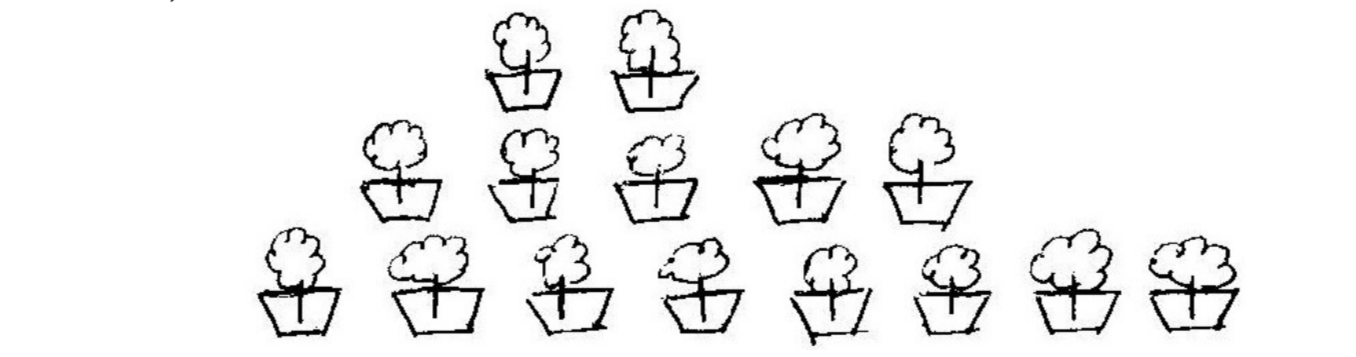
\includegraphics[width=\columnwidth]{figs/ap/Plant.png}
			\caption{Plants}
			\label{fig:Plants}
		\end{figure}
		Based on the above, answer the following questions :
		\begin{enumerate}[label=(\roman*)]
\item How many pots were placed in the $7^{th}$ row ?
				\begin{enumerate}[label=\Alph*]
					 \item $20$
					 \item $23$
					 \item $77$
					 \item $29$
				\end{enumerate}
 \item If Roshini wants to place $100$ pots in total, then total number of rows formed in the arrangement will be ?
				\begin{enumerate}[label=\Alph*]
					 \item $8$
					 \item $9$
					 \item $10$
					 \item $12$
				\end{enumerate}
 \item How many pots are placed in the last row ?
				\begin{enumerate}[label=\Alph*]
					 \item $20$
					 \item $23$
					 \item $26$
					 \item $29$
				\end{enumerate}
			\hfill (2021) \item If Roshini ha sufficient space for $12$ rows, then how many total number of pots are placed by her wih the same arrangement ?
				\begin{enumerate}[label=\Alph*]
					 \item $222$
					 \item $155$
					 \item $187$
					 \item $313$
				\end{enumerate}
		\end{enumerate} 
\hfill (2021)
	 \item The sum of the first $4$ terms of an A.P. is zero and its $4^{th}$ term is $2$. Find the A.P.
	\hfill (2021) \item If the sum of the first $n$ terms of an A.P. is given by $S_n = 4n - n^2$, then find its $n^{th}$ term. Hence, find the $25^{th}$ term and the sum if the first 25 terms of this A.P.
\hfill (2021)
	 \item Find the mean of first $10$ composite numbers.
	\hfill (2021) \item If $S_n$ denotes the sum of first $n$ terms of an A.P., prove that $S_{12} = 3(S_8 - S_4)$.
	\hfill (2021) \item After how many decimal places will the decimal expansion of the rational number $\frac{14587}{1250}$ terminate ?			
\hfill (2021)
	 \item If the $6^{th}$ and $14^{th}$ terms of an A.P. are 29 and 69 respectively, then find the $10^{th}$ term of the A.P.
	\hfill (2021) \item If the first three consecutive terms of an A.P. are $3y-1, 3y+5$ and $5y+1$ find the value of y. 
\hfill (2021)
 \item Which of the following is not an A.P.? 
\begin{enumerate}[label =(\Alph*)]
               \item $-1.2,0.8,2.8,\dots$ 
	        \item $3,3+\sqrt2,3+2\sqrt2,3+3\sqrt2,\dots$ 
	        \item $\frac{4}{3},\frac{7}{3},\frac{9}{3},\frac{12}{3},\dots$ 
	        \item $\frac{-1}{5},\frac{-2}{5},\frac{-3}{5},\dots$ 
\end{enumerate}

\hfill (2020) \item Find the sum of the first $100$ natural numbers.	
	\hfill (2020)
 \item Find the Sum:
\begin{align*}
	\brak{-5} + \brak{-8} + \brak{-11} + \dots + \brak{-230}
\end{align*}
\hfill (2020)

 \item Find the number of terms in the A.P. :
\begin{align*}
    18,15\frac{1}{2},13, ...,-47.
\end{align*}

\hfill (2019) \item Determine the A.P. whose third term is $16$ and $7^{th}$ term exceeds the $5^{th}$ term by $12$.

\hfill (2019) \item Find the value of $x$, when in the A.P. given below
\begin{align*}
2 + 6 + 10 + ... + x = 1800.    
\end{align*}

\hfill (2019) \item Which term of the A.P. $-4, - 1, 2, ... $is$ 101$?

\hfill (2019) \item In an A.P., the first term is $- 4$, the last term is $29$ and the sum of all its terms is $150$. Find its common difference.
\hfill (2019)

\hfill (2019) \item Find the $21^{st}$ term of the A.P. $-4 \frac{1}{2},-3,-1\frac{1}{2},...$

\hfill (2019) \item Find the common difference of the Arithmetic Progression (A.P.) 
\begin{align*}
\frac{1}{a} , \frac{3-a}{3a},\frac{3-2a}{3a} , . . (a \neq 0)
\end{align*}

\hfill (2019) \item Which term of the Arithmetic Progression $-7, -12, -17, -22, ... $ will be $-82$ ? Is $-100$ any term of the A.P. ? Give reason for your answer.

\hfill (2019) \item How many terms of the Arithmetic Progression $45, 39, 33, ... $must be taken so that their sum is $180$ ? Explain the double answer.

\hfill (2019) \item Find after how many places of decimal the decimal form of the number $\frac {27}{2^3.5^4.3^2}$ will terminate.

\hfill (2019) \item Find the sum of first $10$ multiples of $6$

\hfill (2019) \item If $m$ times the $m^{th}$ term of an Arithmetic Progression is equal to $n$ times
its $n^{th}$ term and $m \neq n$, show that the $\brak{m + n}^{th}$ term of the A.P is zero

\hfill (2019) \item The sum of the first three numbers in an Arithmetic Progression is $18$. If the product of the first and the third term is $5$ times the common
difference, find the three numbers.
 \item Find the sum of all the two digit numbers which leave the remainder $2$ when divided by $5$.

\hfill (2019) \item If in an A.P ., $a=15$,$d=-3$ and $a_n=0$, then find the value of $n$.

\hfill (2019) \item If ${S_n}$, the sum of the first ${n}$ terms of an A.P. is given by ${S_n = 2n^2 + n}$,then find its $n^{th}$ term. 

\hfill (2019) \item If the $17^{th}$ term of an A.P. exceeds its $10^{th}$ term by $7$, find the common difference.

\hfill (2019) \item If the sum of the first $p$ terms of an A.P. is $q$ and the sum of the first $q$ terms is $p$; then show that the sum of the first $\brak{p + q}$ terms is $\cbrak {-\brak {p + q}}$.

\hfill (2019) \item Write the common difference of the A.P.${\sqrt3} , {\sqrt12} , {\sqrt27} , {\sqrt48}$ , ... 

\hfill (2019) \item In an A.P., the $n^{th}$ term is ${\frac{1}{m}}$ and the $m^{th}$ term is $\frac{1}{n}$. Find 
\begin{enumerate}
      \item  $\brak{mn}^{th}$term  ,
      \item sum of first $\brak{mn}$ terms.
\end{enumerate}
\hfill (2019)

 \item The first term of an AP is 3, the last term is 83 and the sum of all its terms is 903. Find the number of terms and the common difference of the AP.
\hfill (2019) \item If the sum of first $n$ terms of an $AP$ is $n^2$, then find its $10$th term.
\hfill (2019) \item Which term of the $AP$ $3, 15, 27, 39, ....$ will be $120$ more than its $21$st term?
\hfill (2019) \item If $S_n$ ,the sum of first $n$ terms of an $AP$ is given by $S_n=3n^2-4n$, find the $n$th term.
\hfill (2019) \item If the sum of first four terms of an $AP$ is $40$ and that of first $14$ terms is $280$. Find the sum of its first $n$ terms.
\hfill (2019)

			 \item In an $AP$, if the common difference $(d) = -4$, and the seventh term$(a_7)$ is $4$, then find the first term.		
			\hfill (2018) \item The sum of four consecuive numbers in an AP is $32$ and the ratio of the product of the first and the last term to the product of two middle term is $7:15$. Find the numbers.
	\hfill (2018) \item Find the sum of $8$ multiples of $3$.
\hfill (2018)

			 \item In an $AP$, if the common difference $(d) = -4$, and the seventh term$(a_7)$ is $4$, then find the first term.		
			\hfill (2018) \item The sum of four consecuive numbers in an AP is $32$ and the ratio of the product of the first and the last term to the product of two middle term is $7:15$. Find the numbers.

	\hfill (2018) \item Find the sum of $8$ multiples of $3$.
\hfill (2018)
 \item The $5^{th}$ and $15^{th}$ terms of an A.P. are $13$ and $-17$ respectively. Find the sum of first $21$ terms of the A.P.
\hfill (2018)

 \item The sum of the first $n$ terms of an A.P. is $5n^{2}+3n$. If its $m^{th}$ terms is $168$, find the value of $m$. Also find the $20^{th}$ term of the A.P.
\hfill (2018) \item The $4^{th}$ and the last terms of an A.P. are $11$ and $89$ respectively. If there are $30$ terms in the A.P., find the A.P and its $23^{rd}$ term.
\hfill (2018) \item Write the $m^{th}$ term of the A.P. $\dfrac{1}{k}$,$\dfrac{1+k}{k}$,$\dfrac{1+2k}{k}$,........
\hfill (2018)
\end{enumerate}


\subsection{JEE}
\begin{enumerate}[label=\thesubsection.\arabic*,ref=\thesubsection.\theenumi,itemsep=1pt]
 \item In an AP, if d=2, n=5 and $a_n=0$, then value of a is
    \begin{enumerate}
         \item 10
         \item 5
         \item -8
         \item 8
    \end{enumerate}
    \hfill (10, 2011) \item Find whether -150 is a term of the AP 17, 12, 7, 2,....?
    \hfill (10, 2011) \item Find the value of the middle term of the following AP :\[- 6, -2, 2,........, 58.\]
   \hfill (10, 2011) \item Determine the AP whose fourth term is 18 and the difference of the ninth term from the fifteenth term is 30.
\hfill (10, 2011) \item Find how many two-digit numbers are divisible by $6$.
 How many multiples of $4$ lie between $10$ and $250$ ? Also find their sum.
    \hfill (10, 2011)
         \item The ratio of the $11$\textsuperscript{th} term to $17$\textsuperscript{th} term of an A.P. is $3:4$. Find the ratio of $5$\textsuperscript{th} to $21$\textsuperscript{th} of the same A.P. Also, find the ratio of the sum of first $5$ terms to that of first $21$ terms
        \hfill (10, 2023) \item $250$ logs are stacked in the following manner:
        $22$ logs in the bottom row , $21$ in the next row, $20$ in the row next to it and so on. In how many rows are the $250$ logs placed and how many logs are there in top row ?
\hfill (10, 2023)
 \item If $-\frac{5}{7}$, $a$, $2$ are consecutive terms in an Arthimetic Progression, then the value of $a$ is 
    \begin{enumerate}
\item $\frac{9}{7}$
 \item $\frac{9}{14}$
 \item $\frac{19}{7}$
 \item $\frac{19}{14}$
    \end{enumerate}
    \hfill (10, 2022) \item Find the sum of first $16$ terms of an Arithmetic Progression whose $4^{\text{th}}$ and $9^{\text{th}}$ terms are $-15$ and $-30$ respectively.
    
        \hfill (10, 2022) \item If the sum of first $14$ terms of an Arithmetic Progression is $1050$ and its fourth term is $40$, find its $20^{\text{th}}$ term.

     \item 
    \begin{enumerate}
         \item Find the sum of the first twelve $2$-digit numbers which are 
multiples of $6$.

         \item In an AP, if $a_2=26$ and $a _ {15} = -26$, then write the AP.
        \end{enumerate}
         \item In Mathematics, relations can be expressed in various ways. The 
matchstick patterns are based on linear relations. Different strategies 
can be used to calculate the number of matchsticks used in different 
		\figref{fig:ap} 
 \\One such pattern is shown below. Observe the pattern and answer the 
following questions using Arithmetic Progression :
\begin{figure}[H]
    \centering
	\includegraphics[width=\columnwidth]{figs/ap/ap.jpg}
	\caption{patterns of Figure1, figure2 ,figure3}
    \label{fig:ap}
\end{figure}
    \begin{enumerate}
	 \item Write the AP for the number of triangles used in the \figref{fig:ap}. Also, 
write the nth term of this AP.
 \item Which figure has $61$ matchsticks ? 
    \end{enumerate} 

    \hfill (10, 2022) 
 \item In an A.P. if the sum of third and seventh term is zero, find its $5^{\text{th}}$ term.
        \hfill (10, 2022)
  \item Determine the AP whose third term is $5$ and seventh term is $9$.
        \hfill (10, 2022) \item Find the sum of the first $20$ terms of an A.P. whose $n^{\text{th}}$ term is given as $a_n=5-2n$
        \hfill (10, 2022) \item Find the common difference 'd' of an AP whose first term is $10$ and the sum of the first $14$ terms is $1505$.

        \hfill (10, 2022) \item For what value of 'n', are the $n^{\text{th}}$ terms of the APs: $9,7,5,\dots$ and $15,12,9,\dots$ the same?
    \hfill (10, 2022)
	 \item Write the common difference of the A.P. :$\frac{1}{5}, \frac{4}{5}, \frac{7}{5}, \frac{10}{5}, \cdots$

	\hfill (2021) \item Find the $8^{th}$ term of the A.P. whose first term is $-2$ and common difference is $3$.
	\hfill (2021) \item
	Roshini being a plant lover decides to start a nursery. She bought few plants with pots.She placed the pots in such a way that the number of pots in the first row is $2$, in the second is $5$, in the third row is $8$ and so on.
		\begin{figure}[h]
			\centering	
			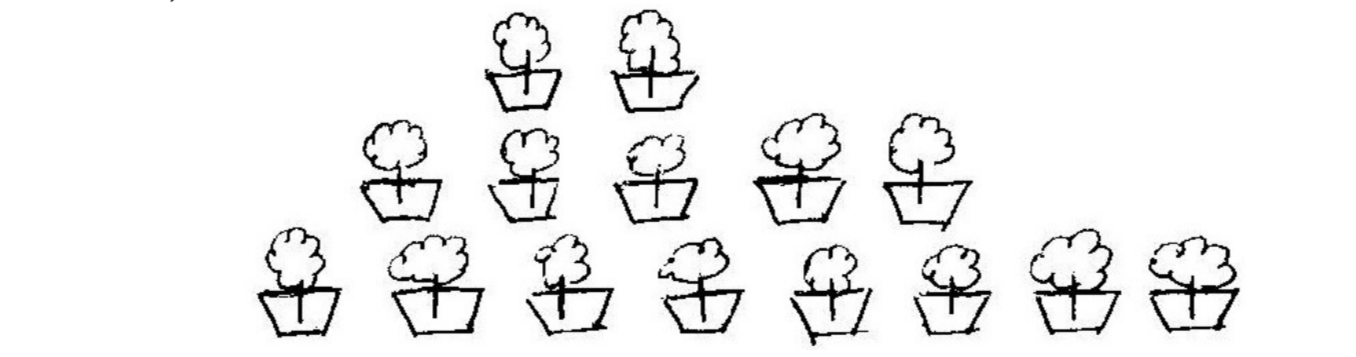
\includegraphics[width=\columnwidth]{figs/ap/Plant.png}
			\caption{Plants}
			\label{fig:Plants}
		\end{figure}
		Based on the above, answer the following questions :
		\begin{enumerate}[label=(\roman*)]
\item How many pots were placed in the $7^{th}$ row ?
				\begin{enumerate}[label=\Alph*]
					 \item $20$
					 \item $23$
					 \item $77$
					 \item $29$
				\end{enumerate}
 \item If Roshini wants to place $100$ pots in total, then total number of rows formed in the arrangement will be ?
				\begin{enumerate}[label=\Alph*]
					 \item $8$
					 \item $9$
					 \item $10$
					 \item $12$
				\end{enumerate}
 \item How many pots are placed in the last row ?
				\begin{enumerate}[label=\Alph*]
					 \item $20$
					 \item $23$
					 \item $26$
					 \item $29$
				\end{enumerate}
			\hfill (2021) \item If Roshini ha sufficient space for $12$ rows, then how many total number of pots are placed by her wih the same arrangement ?
				\begin{enumerate}[label=\Alph*]
					 \item $222$
					 \item $155$
					 \item $187$
					 \item $313$
				\end{enumerate}
		\end{enumerate} 
\hfill (2021)
	 \item The sum of the first $4$ terms of an A.P. is zero and its $4^{th}$ term is $2$. Find the A.P.
	\hfill (2021) \item If the sum of the first $n$ terms of an A.P. is given by $S_n = 4n - n^2$, then find its $n^{th}$ term. Hence, find the $25^{th}$ term and the sum if the first 25 terms of this A.P.
\hfill (2021)
	 \item Find the mean of first $10$ composite numbers.
	\hfill (2021) \item If $S_n$ denotes the sum of first $n$ terms of an A.P., prove that $S_{12} = 3(S_8 - S_4)$.
	\hfill (2021) \item After how many decimal places will the decimal expansion of the rational number $\frac{14587}{1250}$ terminate ?			
\hfill (2021)
	 \item If the $6^{th}$ and $14^{th}$ terms of an A.P. are 29 and 69 respectively, then find the $10^{th}$ term of the A.P.
	\hfill (2021) \item If the first three consecutive terms of an A.P. are $3y-1, 3y+5$ and $5y+1$ find the value of y. 
\hfill (2021)
 \item Which of the following is not an A.P.? 
\begin{enumerate}[label =(\Alph*)]
               \item $-1.2,0.8,2.8,\dots$ 
	        \item $3,3+\sqrt2,3+2\sqrt2,3+3\sqrt2,\dots$ 
	        \item $\frac{4}{3},\frac{7}{3},\frac{9}{3},\frac{12}{3},\dots$ 
	        \item $\frac{-1}{5},\frac{-2}{5},\frac{-3}{5},\dots$ 
\end{enumerate}

\hfill (2020) \item Find the sum of the first $100$ natural numbers.	
	\hfill (2020)
 \item Find the Sum:
\begin{align*}
	\brak{-5} + \brak{-8} + \brak{-11} + \dots + \brak{-230}
\end{align*}
\hfill (2020)

 \item Find the number of terms in the A.P. :
\begin{align*}
    18,15\frac{1}{2},13, ...,-47.
\end{align*}

\hfill (2019) \item Determine the A.P. whose third term is $16$ and $7^{th}$ term exceeds the $5^{th}$ term by $12$.

\hfill (2019) \item Find the value of $x$, when in the A.P. given below
\begin{align*}
2 + 6 + 10 + ... + x = 1800.    
\end{align*}

\hfill (2019) \item Which term of the A.P. $-4, - 1, 2, ... $is$ 101$?

\hfill (2019) \item In an A.P., the first term is $- 4$, the last term is $29$ and the sum of all its terms is $150$. Find its common difference.
\hfill (2019)

\hfill (2019) \item Find the $21^{st}$ term of the A.P. $-4 \frac{1}{2},-3,-1\frac{1}{2},...$

\hfill (2019) \item Find the common difference of the Arithmetic Progression (A.P.) 
\begin{align*}
\frac{1}{a} , \frac{3-a}{3a},\frac{3-2a}{3a} , . . (a \neq 0)
\end{align*}

\hfill (2019) \item Which term of the Arithmetic Progression $-7, -12, -17, -22, ... $ will be $-82$ ? Is $-100$ any term of the A.P. ? Give reason for your answer.

\hfill (2019) \item How many terms of the Arithmetic Progression $45, 39, 33, ... $must be taken so that their sum is $180$ ? Explain the double answer.

\hfill (2019) \item Find after how many places of decimal the decimal form of the number $\frac {27}{2^3.5^4.3^2}$ will terminate.

\hfill (2019) \item Find the sum of first $10$ multiples of $6$

\hfill (2019) \item If $m$ times the $m^{th}$ term of an Arithmetic Progression is equal to $n$ times
its $n^{th}$ term and $m \neq n$, show that the $\brak{m + n}^{th}$ term of the A.P is zero

\hfill (2019) \item The sum of the first three numbers in an Arithmetic Progression is $18$. If the product of the first and the third term is $5$ times the common
difference, find the three numbers.
 \item Find the sum of all the two digit numbers which leave the remainder $2$ when divided by $5$.

\hfill (2019) \item If in an A.P ., $a=15$,$d=-3$ and $a_n=0$, then find the value of $n$.

\hfill (2019) \item If ${S_n}$, the sum of the first ${n}$ terms of an A.P. is given by ${S_n = 2n^2 + n}$,then find its $n^{th}$ term. 

\hfill (2019) \item If the $17^{th}$ term of an A.P. exceeds its $10^{th}$ term by $7$, find the common difference.

\hfill (2019) \item If the sum of the first $p$ terms of an A.P. is $q$ and the sum of the first $q$ terms is $p$; then show that the sum of the first $\brak{p + q}$ terms is $\cbrak {-\brak {p + q}}$.

\hfill (2019) \item Write the common difference of the A.P.${\sqrt3} , {\sqrt12} , {\sqrt27} , {\sqrt48}$ , ... 

\hfill (2019) \item In an A.P., the $n^{th}$ term is ${\frac{1}{m}}$ and the $m^{th}$ term is $\frac{1}{n}$. Find 
\begin{enumerate}
      \item  $\brak{mn}^{th}$term  ,
      \item sum of first $\brak{mn}$ terms.
\end{enumerate}
\hfill (2019)

 \item The first term of an AP is 3, the last term is 83 and the sum of all its terms is 903. Find the number of terms and the common difference of the AP.
\hfill (2019) \item If the sum of first $n$ terms of an $AP$ is $n^2$, then find its $10$th term.
\hfill (2019) \item Which term of the $AP$ $3, 15, 27, 39, ....$ will be $120$ more than its $21$st term?
\hfill (2019) \item If $S_n$ ,the sum of first $n$ terms of an $AP$ is given by $S_n=3n^2-4n$, find the $n$th term.
\hfill (2019) \item If the sum of first four terms of an $AP$ is $40$ and that of first $14$ terms is $280$. Find the sum of its first $n$ terms.
\hfill (2019)

			 \item In an $AP$, if the common difference $(d) = -4$, and the seventh term$(a_7)$ is $4$, then find the first term.		
			\hfill (2018) \item The sum of four consecuive numbers in an AP is $32$ and the ratio of the product of the first and the last term to the product of two middle term is $7:15$. Find the numbers.
	\hfill (2018) \item Find the sum of $8$ multiples of $3$.
\hfill (2018)

			 \item In an $AP$, if the common difference $(d) = -4$, and the seventh term$(a_7)$ is $4$, then find the first term.		
			\hfill (2018) \item The sum of four consecuive numbers in an AP is $32$ and the ratio of the product of the first and the last term to the product of two middle term is $7:15$. Find the numbers.

	\hfill (2018) \item Find the sum of $8$ multiples of $3$.
\hfill (2018)
 \item The $5^{th}$ and $15^{th}$ terms of an A.P. are $13$ and $-17$ respectively. Find the sum of first $21$ terms of the A.P.
\hfill (2018)

 \item The sum of the first $n$ terms of an A.P. is $5n^{2}+3n$. If its $m^{th}$ terms is $168$, find the value of $m$. Also find the $20^{th}$ term of the A.P.
\hfill (2018) \item The $4^{th}$ and the last terms of an A.P. are $11$ and $89$ respectively. If there are $30$ terms in the A.P., find the A.P and its $23^{rd}$ term.
\hfill (2018) \item Write the $m^{th}$ term of the A.P. $\dfrac{1}{k}$,$\dfrac{1+k}{k}$,$\dfrac{1+2k}{k}$,........
\hfill (2018)
\end{enumerate}


\section{Geometric Progression}
\subsection{Formulae}
\begin{enumerate}[label=\thesubsection.\arabic*,ref=\thesubsection.\theenumi]
	\item The $n^{th}$ term of a GP is given by 
\begin{align}
	\label{eq:gp-nthterm}
	x(n)= x(0)r^n, n = 0,1,2, \dots 
\end{align}
where $r$
		is defined to be the {\em common ratio}.
\item Find the sum 
\begin{align}
	\label{eq:gp-sum10}
	S = 1 + 2 + 2^2 + 2^3 + 2^4
\end{align}
	\solution
Mulitpying the sum in
	\eqref{eq:gp-sum10}
	as
\begin{align}
	\label{eq:gp-sum10-rev}
	2S =  2 + 2^2 + 2^3 + 2^4+ 2^5
\end{align}
and  subtracting
	\eqref{eq:gp-sum10}
	from
	\eqref{eq:gp-sum10-rev},
\begin{align}
	\label{eq:gp-sum10-add}
	S = 2^5 - 1
\end{align}
\item The sum of a GP is 
\begin{align}
	 y(n)=\sum_{k=0}^{n-1}x(k)  
	= x(0)\brak{\frac{1-r^{n}}{1-r}}
	\label{eq:gp-sumn}
\end{align}
\item  For an infinite GP, 
\begin{align}
	\lim_{r\to\infty}	y(n) = 
	 \brak{\frac{x(0)}{1-r}},\quad \abs{r} < 1
	\label{eq:gp-sumn-infty}
\end{align}
\end{enumerate}

\subsection{NCERT}
\begin{enumerate}[label=\thesubsection.\arabic*.,ref=\thesubsection.\theenumi]
\item Find the $20^{th}$ and $n^{th}$ terms of the GP: $\frac{5}{2}, \frac{5}{4}, \frac{5}{8},\dots, $
	\\
	\solution
\begin{align}
	a_0 &= \frac{5}{2}, r = \frac{1}{2}
	\\
	\implies a_{19} &=\frac{5}{2}\brak{\frac{1}{2}}^{19}=\frac{5}{2^{20}}
	\\
	a_{n-1} &= \frac{5}{2^n}
\end{align}
using
	\eqref{eq:gp-nthterm}.
\item The $5^{th}$, $8^{th}$ and $11^{th}$ terms of a GP  are $p, q$ and $s$, respectively. Show that 
$q^2 = ps$.
\item The $4^{th}$ term of a GP  is square of its second term, and the first term is -3. Determine its $7^{th}$ term.
	\\
	\solution  From the given information, 
\begin{align}
	a_3 &= a_1^2, a_0 = -3
	\\
	\implies a_0r^3&= a_0^2r^2
	\\
	\text{or, } r &= a_0
	\\
	\therefore a_6 &= a_0^7= \brak{-3}^7
\end{align}
\item Which term of the following sequences
\begin{enumerate}
	\item 2, 2 $\sqrt{2}$, 4,\dots,  is 128 ?
	\item $\sqrt{3}, 3, 3\sqrt{3},\dots,$  is 729?
	\item $\frac{1}{3}, \frac{1}{9}, \frac{1}{27}, \dots,$  is $\frac{1}{19683}$?
\end{enumerate}
	\solution
\begin{enumerate}
	\item 
\begin{align}
	a_0&= 2, r = \sqrt{2}
	\\
	a_n &= a_0r^n = 128
	\\
		\implies 2\brak{\sqrt{2}}^n &= 128
		\\
		\text{or, } n &= 2\brak{\frac{\log 128}{\log 2}-1}=12
\end{align}
\end{enumerate}
\item For what values of $x$, the numbers $-\frac{2}{7}, x, -\frac{7}{2}$ are in GP?
\\
	Find the sum to indicated number of terms in each of the geometric progressions.
\item 0.15, 0.015, 0.0015,\dots,  20 terms.
\item $\sqrt{7}, \sqrt{21}, \sqrt[3]{7}, \dots,  n$ terms.
\item $1, -a, a^2, -a^2, a^3,\dots,  n$ terms $\brak{a \neq -1}$.
\item $x^3, x^5, x^7,\dots,  n$ terms $\brak{x \neq \pm 1}$.
\item Evaluate $$\sum _{k=1}^{11} \brak{2 + 3^k}.$$
	\\
	\solution  The summation can be expressed as
\begin{align}
\sum _{k=1}^{11} 2 +\sum _{k=1}^{11} 3^k
	=2\times 11 +\sum _{k=0}^{10} 3^{k+1}
	\\
	=22+3\sum _{k=0}^{10} 3^{k}=22+3\brak{\frac{3^{11}-1}{2}}
\end{align}
\item The sum of first three terms of a GP  is $\frac{39}{10}$ and their product is 1. Find the 
common ratio and the terms.
	\\
	\solution
\begin{align}
	a_0\brak{1+r+r^2}=\frac{39}{10}
	\\
	a_0^3r^3=1 \implies a_0r = 1
	\\
	\therefore
	{10}\brak{1+r+r^2}={39}r
\end{align}
yielding the quadratic
\begin{align}
	{10}r^2-29r + 10=0
	\\
	\implies \brak{5r - 2}\brak{2r-5}=0
	\text{or, }
	r = \frac{5}{2},\frac{2}{5}
\end{align}
\item How many terms of GP  3, $3^2, 3^3$, \dots,  are needed to give the sum 120?
\item The sum of first three terms of a GP  is 16 and the sum of the next three terms is 128. Determine the first term, the common ratio and the sum to $n$ terms of the GP 
\item Given a GP  with $a = 729$ and $7^{th}$ term 64, determine $S_7$.
\item If the $4^{th}$, $10^{th}$ and $16^{th}$ terms of a GP  are $x, y$ and $z$, respectively. Prove that $x, y, z$ are in GP.
\item Find the sum to $n$ terms of the sequence, $8, 88, 888, 8888, \dots$. 
\item Find the sum of the products of the corresponding terms of the sequences 2, 4, 8, 16, 32, and 128, 32, 8, 2, $\frac{1}{2}$.
\item Show that the products of the corresponding terms of the sequences $a, ar, ar^2,\dots,  ar^{n-1}$ and $A, AR, AR^2,\dots,  AR^{n -1}$ form a GP  and find the common ratio.
\item If the $p^{th}, q^{th}$ and $r^{th}$ terms of a GP  are $a, b$ and $c$, respectively. Prove that 
$$a^{q-r} b^{r-p} c^{p-q} = 1.$$
\item If the first and the $n^{th}$ term of a GP  are $a$ and $b$, respectively, and if $P$ is the product of $n$ terms, prove that $P^2 = \brak{ab}^n.$
\item If $a, b, c$ and $d$ are in GP  show that $\brak{a^2 + b^2 + c^2}\brak{b^2 + c^2 + d^2} = \brak{ab + bc + cd}^2.$
\item The number of bacteria in a certain culture doubles every hour. If there were 30 bacteria present in the culture originally, how many bacteria will be present at the end of $2^{nd}$ hour, 
$4^{th}$ hour and $n^{th}$ hour ?
\item What will Rs 500 amount to in 10 years after its deposit in a bank which pays annual interest rate of 10\% compounded annually?
\item If AM  and GM  of roots of a quadratic equation are 8 and 5, respectively, then obtain the quadratic equation.
\item If $f$ is a function satisfying $$f\brak{x +y} = f\brak{x} f\brak{y} \forall x,y \in N$$ such that 
	$$f\brak{1} = 3\text{ and }\sum_{x = 1}^n f\brak{x} = 120,$$ find the value of $n$.
\item The sum of some terms of GP  is 315 whose first term and the common ratio are 5 and 2, respectively. Find the last term and the number of terms.
\item  The first term of a GP  is 1. The sum of the third term and fifth term is 90. Find the common ratio of the GP.
\item The sum of three numbers in GP  is 56. If we subtract 1, 7, 21 from these numbers in that order, we obtain an arithmetic progression. Find the numbers.
\item A GP  consists of an even number of terms. If the sum of all the terms is 5 times the sum of terms occupying odd places, then find its common ratio.
\item  The sum of the first four terms of an AP  is 56. The sum of the last four terms is 112. If its first term is 11, then find the number of terms.
\item If $$\frac{a+bx}{a-bx} = \frac{b+cx}{b-cx} = \frac{c+dx}{c-dx}\brak{x \neq 0},$$ then show that $a, b, c$ and $d$ are in GP.
\item Let $S$ be the sum, $P$ the product and $R$ the sum of reciprocals of $n$ terms in a GP.  Prove that $P^2R^n = S^n.$ 
\item The $p^{th}, q^{th}$ and $r^{th}$ terms of an AP  are $a, b, c,$ respectively. Show that 
$$\brak{q - r }a + \brak{r - p }b + \brak{p - q }c = 0.$$
\item If $$a\brak{\frac{1}{b}+\frac{1}{c}}, b\brak{\frac{1}{c}+\frac{1}{a}}, c\brak{\frac{1}{a}+\frac{1}{b}}$$ are in AP, prove that $a, b, c$ are in AP 
\item If $a, b, c, d$ are in GP  prove that $$\brak{a^n + b^n}, \brak{b^n + c^n}, \brak{c^n + d^n}$$ are in GP. 
\item If $a$ and $b$ are the roots of $$x^2 - 3x + p = 0$$ and $c, d$ are roots of $$x^2 - 12x + q = 0,$$ where $a, b, c, d$ form a GP,  prove that $$\brak{q + p} : \brak{q - p} = 17:15.$$
\item The ratio of the AM  and GM  of two positive numbers $a$ and $b$, is $m : n$. Show that 
$$a:b = \brak{m+\sqrt{m^2 - n^2}}:\brak{m - \sqrt{m^2 - n^2}}.$$
\item If $a, b, c$ are in AP; $b, c, d$ are in GP  and $$\frac{1}{c}, \frac{1}{d}, \frac{1}{e}$$ are in AP  prove that $a, c, e$ are in GP.
\item Find the sum of the following series up to $n$ terms
\begin{enumerate}
\item 5 + 55 +555 + \dots, 
\item .6 + .66 + .666+\dots 
\end{enumerate}
\item A person writes a letter to four of his friends. He asks each one of them to copy
the letter and mail to four different persons with instruction that they move the
chain similarly. Assuming that the chain is not broken and that it costs 50 paise to
mail one letter. Find the amount spent on the postage when $8^{th}$ set of letter is
mailed. 
\item A manufacturer reckons that the value of a machine,  which costs him Rs. 15625,  will depreciate each year by 20\%. Find the estimated value at the end of 5 years. 
\item 150 workers were engaged to finish a job in a certain number of days. 4 workers dropped out on second day,  4 more workers dropped out on third day and so on.It took 8 more days to finish the work. Find the number of days in which the work was completed.
	\item Find the $10^{th}$ and $n^{th}$ and  terms of the GP: $5, 25, 125, \dots$
	\item Which term of the GP: $2, 8, 32, \dots $ upto $n$ terms is 131072.
	\item In a GP the $3^{rd}$ term is 24 and the $6^{th}$ term is 192.  Find the $10^{th}$ term.
	\item Find the sum of the first $n$ terms and the sum of the first 5 terms of the series 
		$$ 1 + \frac{2}{3}+\frac{4}{9}+\dots$$
	\item How many terms of the GP: 
		$$ 3 + \frac{3}{2}+\frac{3}{4}+\dots$$
		are needed to give the sum $\frac{3069}{512}$.
	\item The sum of the first 3 terms of a GP is 
$\frac{13}{12}$ and their product is -1.  Find the common ratio and the terms.
\item Find the sum of the sequence $7, 77, 777, \dots$ to $n$ terms.
\item A person has 2 parents, 4 grandparents, 8 great grand parents and so on.  Find the number of his ancestors during the ten generations preceeding his own.
\item Insert 3 numbers between 1 and 256 so that the resulting sequence is a GP.
\item If the AM and GM of two positive numbers $a$ and $b$ are 10 and 8 respectively, find the numbers.
\item Find the $12^{th}$ term of a GP  whose $8^{th}$ term is 192 and the common ratio is 2.
\item Find a GP  for which sum of the first two terms is -4 and the fifth term is 4 times the third term.
\item Find four numbers forming a geometric progression in which the third term is greater than the first term by 9, and the second term is greater than the $4^{th}$ by 18.
\item Show that the ratio of the sum of first $n$ terms of a GP  to the sum of terms from $\brak{n+1}^{th}$ to $\brak{2n}^{th}$ term is $\frac{1}{r^n}$.
\item Insert two numbers between 3 and 81 so that the resulting sequence is GP 
\item Find the value of $n$ so that $$\frac{a^{n + 1} + b^{n + 1}}{a^n + b^n}$$ may be the geometric mean between $a$ and $b$.
\item The sum of two numbers is 6 times their geometric mean, show that numbers are in the ratio $$\brak{3+2\sqrt{2}}:\brak{3-2\sqrt{2}}.$$
\item If $A$ and $G$ be AM  and GM, respectively between two positive numbers, prove that the numbers are $$A \pm \sqrt{\brak{A+G}\brak{A-G}}.$$
\item If the $p^{th}, q^{th}, r^{th}$ and $s^{th}$ terms of an AP are in GP, then show that $\brak{p-q},\brak{q-r},\brak{r-s}$ are also in GP.
\item If $a,b,c$ are in GP and $a^{\frac{1}{x}}b^{\frac{1}{y}}c^{\frac{1}{z}}$, prove that $x,y,z$ are in AP.
\item If $a, b, c, d, p$ are different real numbers such that 
	$$\brak{a^2+b^2+c^2}p^2-2\brak{ab+bc+cd}p+\brak{b^2+c^2+d^2} \le 0,$$ then show that $a,b,c$ and $d$ are in GP.
\item If $p,q,r$ are in GP and the equations 
	$$px^2+qx+r = 0, \quad dx^2+2ex+f = 0$$
	have a common root, then show that
	$$\frac{d}{p},\frac{e}{q},\frac{f}{r}$$ are in AP.
\end{enumerate}

\subsection{JEE}
\begin{enumerate}[label=\thesubsection.\arabic*.,ref=\thesubsection.\theenumi]
\item Find the $20^{th}$ and $n^{th}$ terms of the GP: $\frac{5}{2}, \frac{5}{4}, \frac{5}{8},\dots, $
	\\
	\solution
\begin{align}
	a_0 &= \frac{5}{2}, r = \frac{1}{2}
	\\
	\implies a_{19} &=\frac{5}{2}\brak{\frac{1}{2}}^{19}=\frac{5}{2^{20}}
	\\
	a_{n-1} &= \frac{5}{2^n}
\end{align}
using
	\eqref{eq:gp-nthterm}.
\item The $5^{th}$, $8^{th}$ and $11^{th}$ terms of a GP  are $p, q$ and $s$, respectively. Show that 
$q^2 = ps$.
\item The $4^{th}$ term of a GP  is square of its second term, and the first term is -3. Determine its $7^{th}$ term.
	\\
	\solution  From the given information, 
\begin{align}
	a_3 &= a_1^2, a_0 = -3
	\\
	\implies a_0r^3&= a_0^2r^2
	\\
	\text{or, } r &= a_0
	\\
	\therefore a_6 &= a_0^7= \brak{-3}^7
\end{align}
\item Which term of the following sequences
\begin{enumerate}
	\item 2, 2 $\sqrt{2}$, 4,\dots,  is 128 ?
	\item $\sqrt{3}, 3, 3\sqrt{3},\dots,$  is 729?
	\item $\frac{1}{3}, \frac{1}{9}, \frac{1}{27}, \dots,$  is $\frac{1}{19683}$?
\end{enumerate}
	\solution
\begin{enumerate}
	\item 
\begin{align}
	a_0&= 2, r = \sqrt{2}
	\\
	a_n &= a_0r^n = 128
	\\
		\implies 2\brak{\sqrt{2}}^n &= 128
		\\
		\text{or, } n &= 2\brak{\frac{\log 128}{\log 2}-1}=12
\end{align}
\end{enumerate}
\item For what values of $x$, the numbers $-\frac{2}{7}, x, -\frac{7}{2}$ are in GP?
\\
	Find the sum to indicated number of terms in each of the geometric progressions.
\item 0.15, 0.015, 0.0015,\dots,  20 terms.
\item $\sqrt{7}, \sqrt{21}, \sqrt[3]{7}, \dots,  n$ terms.
\item $1, -a, a^2, -a^2, a^3,\dots,  n$ terms $\brak{a \neq -1}$.
\item $x^3, x^5, x^7,\dots,  n$ terms $\brak{x \neq \pm 1}$.
\item Evaluate $$\sum _{k=1}^{11} \brak{2 + 3^k}.$$
	\\
	\solution  The summation can be expressed as
\begin{align}
\sum _{k=1}^{11} 2 +\sum _{k=1}^{11} 3^k
	=2\times 11 +\sum _{k=0}^{10} 3^{k+1}
	\\
	=22+3\sum _{k=0}^{10} 3^{k}=22+3\brak{\frac{3^{11}-1}{2}}
\end{align}
\item The sum of first three terms of a GP  is $\frac{39}{10}$ and their product is 1. Find the 
common ratio and the terms.
	\\
	\solution
\begin{align}
	a_0\brak{1+r+r^2}=\frac{39}{10}
	\\
	a_0^3r^3=1 \implies a_0r = 1
	\\
	\therefore
	{10}\brak{1+r+r^2}={39}r
\end{align}
yielding the quadratic
\begin{align}
	{10}r^2-29r + 10=0
	\\
	\implies \brak{5r - 2}\brak{2r-5}=0
	\text{or, }
	r = \frac{5}{2},\frac{2}{5}
\end{align}
\item How many terms of GP  3, $3^2, 3^3$, \dots,  are needed to give the sum 120?
\item The sum of first three terms of a GP  is 16 and the sum of the next three terms is 128. Determine the first term, the common ratio and the sum to $n$ terms of the GP 
\item Given a GP  with $a = 729$ and $7^{th}$ term 64, determine $S_7$.
\item If the $4^{th}$, $10^{th}$ and $16^{th}$ terms of a GP  are $x, y$ and $z$, respectively. Prove that $x, y, z$ are in GP.
\item Find the sum to $n$ terms of the sequence, $8, 88, 888, 8888, \dots$. 
\item Find the sum of the products of the corresponding terms of the sequences 2, 4, 8, 16, 32, and 128, 32, 8, 2, $\frac{1}{2}$.
\item Show that the products of the corresponding terms of the sequences $a, ar, ar^2,\dots,  ar^{n-1}$ and $A, AR, AR^2,\dots,  AR^{n -1}$ form a GP  and find the common ratio.
\item If the $p^{th}, q^{th}$ and $r^{th}$ terms of a GP  are $a, b$ and $c$, respectively. Prove that 
$$a^{q-r} b^{r-p} c^{p-q} = 1.$$
\item If the first and the $n^{th}$ term of a GP  are $a$ and $b$, respectively, and if $P$ is the product of $n$ terms, prove that $P^2 = \brak{ab}^n.$
\item If $a, b, c$ and $d$ are in GP  show that $\brak{a^2 + b^2 + c^2}\brak{b^2 + c^2 + d^2} = \brak{ab + bc + cd}^2.$
\item The number of bacteria in a certain culture doubles every hour. If there were 30 bacteria present in the culture originally, how many bacteria will be present at the end of $2^{nd}$ hour, 
$4^{th}$ hour and $n^{th}$ hour ?
\item What will Rs 500 amount to in 10 years after its deposit in a bank which pays annual interest rate of 10\% compounded annually?
\item If AM  and GM  of roots of a quadratic equation are 8 and 5, respectively, then obtain the quadratic equation.
\item If $f$ is a function satisfying $$f\brak{x +y} = f\brak{x} f\brak{y} \forall x,y \in N$$ such that 
	$$f\brak{1} = 3\text{ and }\sum_{x = 1}^n f\brak{x} = 120,$$ find the value of $n$.
\item The sum of some terms of GP  is 315 whose first term and the common ratio are 5 and 2, respectively. Find the last term and the number of terms.
\item  The first term of a GP  is 1. The sum of the third term and fifth term is 90. Find the common ratio of the GP.
\item The sum of three numbers in GP  is 56. If we subtract 1, 7, 21 from these numbers in that order, we obtain an arithmetic progression. Find the numbers.
\item A GP  consists of an even number of terms. If the sum of all the terms is 5 times the sum of terms occupying odd places, then find its common ratio.
\item  The sum of the first four terms of an AP  is 56. The sum of the last four terms is 112. If its first term is 11, then find the number of terms.
\item If $$\frac{a+bx}{a-bx} = \frac{b+cx}{b-cx} = \frac{c+dx}{c-dx}\brak{x \neq 0},$$ then show that $a, b, c$ and $d$ are in GP.
\item Let $S$ be the sum, $P$ the product and $R$ the sum of reciprocals of $n$ terms in a GP.  Prove that $P^2R^n = S^n.$ 
\item The $p^{th}, q^{th}$ and $r^{th}$ terms of an AP  are $a, b, c,$ respectively. Show that 
$$\brak{q - r }a + \brak{r - p }b + \brak{p - q }c = 0.$$
\item If $$a\brak{\frac{1}{b}+\frac{1}{c}}, b\brak{\frac{1}{c}+\frac{1}{a}}, c\brak{\frac{1}{a}+\frac{1}{b}}$$ are in AP, prove that $a, b, c$ are in AP 
\item If $a, b, c, d$ are in GP  prove that $$\brak{a^n + b^n}, \brak{b^n + c^n}, \brak{c^n + d^n}$$ are in GP. 
\item If $a$ and $b$ are the roots of $$x^2 - 3x + p = 0$$ and $c, d$ are roots of $$x^2 - 12x + q = 0,$$ where $a, b, c, d$ form a GP,  prove that $$\brak{q + p} : \brak{q - p} = 17:15.$$
\item The ratio of the AM  and GM  of two positive numbers $a$ and $b$, is $m : n$. Show that 
$$a:b = \brak{m+\sqrt{m^2 - n^2}}:\brak{m - \sqrt{m^2 - n^2}}.$$
\item If $a, b, c$ are in AP; $b, c, d$ are in GP  and $$\frac{1}{c}, \frac{1}{d}, \frac{1}{e}$$ are in AP  prove that $a, c, e$ are in GP.
\item Find the sum of the following series up to $n$ terms
\begin{enumerate}
\item 5 + 55 +555 + \dots, 
\item .6 + .66 + .666+\dots 
\end{enumerate}
\item A person writes a letter to four of his friends. He asks each one of them to copy
the letter and mail to four different persons with instruction that they move the
chain similarly. Assuming that the chain is not broken and that it costs 50 paise to
mail one letter. Find the amount spent on the postage when $8^{th}$ set of letter is
mailed. 
\item A manufacturer reckons that the value of a machine,  which costs him Rs. 15625,  will depreciate each year by 20\%. Find the estimated value at the end of 5 years. 
\item 150 workers were engaged to finish a job in a certain number of days. 4 workers dropped out on second day,  4 more workers dropped out on third day and so on.It took 8 more days to finish the work. Find the number of days in which the work was completed.
	\item Find the $10^{th}$ and $n^{th}$ and  terms of the GP: $5, 25, 125, \dots$
	\item Which term of the GP: $2, 8, 32, \dots $ upto $n$ terms is 131072.
	\item In a GP the $3^{rd}$ term is 24 and the $6^{th}$ term is 192.  Find the $10^{th}$ term.
	\item Find the sum of the first $n$ terms and the sum of the first 5 terms of the series 
		$$ 1 + \frac{2}{3}+\frac{4}{9}+\dots$$
	\item How many terms of the GP: 
		$$ 3 + \frac{3}{2}+\frac{3}{4}+\dots$$
		are needed to give the sum $\frac{3069}{512}$.
	\item The sum of the first 3 terms of a GP is 
$\frac{13}{12}$ and their product is -1.  Find the common ratio and the terms.
\item Find the sum of the sequence $7, 77, 777, \dots$ to $n$ terms.
\item A person has 2 parents, 4 grandparents, 8 great grand parents and so on.  Find the number of his ancestors during the ten generations preceeding his own.
\item Insert 3 numbers between 1 and 256 so that the resulting sequence is a GP.
\item If the AM and GM of two positive numbers $a$ and $b$ are 10 and 8 respectively, find the numbers.
\item Find the $12^{th}$ term of a GP  whose $8^{th}$ term is 192 and the common ratio is 2.
\item Find a GP  for which sum of the first two terms is -4 and the fifth term is 4 times the third term.
\item Find four numbers forming a geometric progression in which the third term is greater than the first term by 9, and the second term is greater than the $4^{th}$ by 18.
\item Show that the ratio of the sum of first $n$ terms of a GP  to the sum of terms from $\brak{n+1}^{th}$ to $\brak{2n}^{th}$ term is $\frac{1}{r^n}$.
\item Insert two numbers between 3 and 81 so that the resulting sequence is GP 
\item Find the value of $n$ so that $$\frac{a^{n + 1} + b^{n + 1}}{a^n + b^n}$$ may be the geometric mean between $a$ and $b$.
\item The sum of two numbers is 6 times their geometric mean, show that numbers are in the ratio $$\brak{3+2\sqrt{2}}:\brak{3-2\sqrt{2}}.$$
\item If $A$ and $G$ be AM  and GM, respectively between two positive numbers, prove that the numbers are $$A \pm \sqrt{\brak{A+G}\brak{A-G}}.$$
\item If the $p^{th}, q^{th}, r^{th}$ and $s^{th}$ terms of an AP are in GP, then show that $\brak{p-q},\brak{q-r},\brak{r-s}$ are also in GP.
\item If $a,b,c$ are in GP and $a^{\frac{1}{x}}b^{\frac{1}{y}}c^{\frac{1}{z}}$, prove that $x,y,z$ are in AP.
\item If $a, b, c, d, p$ are different real numbers such that 
	$$\brak{a^2+b^2+c^2}p^2-2\brak{ab+bc+cd}p+\brak{b^2+c^2+d^2} \le 0,$$ then show that $a,b,c$ and $d$ are in GP.
\item If $p,q,r$ are in GP and the equations 
	$$px^2+qx+r = 0, \quad dx^2+2ex+f = 0$$
	have a common root, then show that
	$$\frac{d}{p},\frac{e}{q},\frac{f}{r}$$ are in AP.
\end{enumerate}

\section{$Z$ Transform}
\subsection{Formulae}
\begin{enumerate}[label=\thesubsection.\arabic*,ref=\thesubsection.\theenumi]
\item 
	The $Z$-transform of $x(n)$ is defined as
\begin{align}
X(z) = \sum_{n=-\infty}^{\infty}x(n)z^{-n}
\label{eq:ztrans}
\end{align}
\item The unit step function is defined as
\begin{align}
	u(n) = 
	\begin{cases}
		1 & n \ge 0
		\\
		0 & \text{otherwise}
	\end{cases}
	\label{eq:unit-step}
\end{align}
\item For a Geometric progression 
\begin{align}
	       \label{eq:gpn}
	x\brak{n} &=r^nu\brak{n},
	\\
         \implies      X\brak{z} &= \sum_{n=-\infty}^{\infty}x\brak{n}z^{-n}
               =\sum_{n=0}^{\infty}r^nz^{-n}\\
                &=\sum_{n=0}^{\infty}\brak{rz^{-1}}^n\\
               &= \frac{1}{1-rz^{-1}}, \quad \abs{z}>\abs{r} 
	       \label{eq:gpz}
\end{align}
from 
	\eqref{eq:gp-sumn-infty}.
\item 	       Substituting $r = 1$ in \eqref{eq:gpz},
\begin{align}
	u(n) \system{Z}	U(z) = 
                \frac{1}{1-z^{-1}}, \quad \abs{z}>1
	       \label{eq:uz}
\end{align}
\item From 
\eqref{eq:xzder}
	       and 
	       \eqref{eq:uz},
\begin{align}
nu(n) &\system{Z}\frac{z^{-1}}{(1-z^{-1})^{2}}, \quad \abs{z} > 1 
	       \label{eq:uzder}
\end{align}
\item 
From \eqref{eq:xzder}
\begin{align}
	nx(n) \system{Z} -zX^{\prime}(z)
\label{eq:xzder}
\end{align}
yielding
\begin{align}
    n u\brak{n} & \system{Z} \frac{z^{-1}}{\brak{1-z^{-1}}^2} ,   \abs{z} >1 \label{eq:11.9.5.26.2}\\
         n^2 u\brak{n} & \system{Z} \frac{z^{-1}\brak{z^{-1}+1}}{\brak{1-z^{-1}}^3} ,  \abs{z} > 1\label{eq:11.9.5.26.3}\\
         n^3 u\brak{n} & \system{Z} \frac{z^{-1}\brak{1+4z^{-1}+z^{-2}}}{\brak{1-z^{-1}}^4} ,   \abs{z} >1\label{eq:11.9.5.26.4} \\
       n^4 u\brak{n} & \system{Z} \frac{z^{-1}\brak{1+11z^{-1}+11z^{-2}+z^{-3}}}{\brak{1-z^{-1}}^5},\abs{z}>1
	\label{eq:11.9.5.26.5}  
\end{align} 
\item The convolution sum is defined as
\begin{align}
	y(n) &= x(n)* h(n) = \sum_{k=-\infty}^{\infty}x\brak{k}h\brak{n-k}
	\label{eq:conv}
\end{align}
\item 
\begin{align}
	x(n-k) &\system{Z} z^{-k}X(z)
\label{eq:shiftk}
\end{align}
\item Using \eqref{eq:shiftk}:
 \begin{align}
         nu\brak{n-1}&\system{Z} z\frac{2z^{-2}}{\brak{1-z^{-1}}^2}
    \end{align}
 Now , 
    \begin{align}
         \frac{\brak{n-1}}{2}u\brak{n-2} & \system{Z} \frac{z^{-2}}{\brak{1-z^{-1}}^2} \\
         \frac{\brak{n-1}\brak{n-2}}{6}u\brak{n-3}&\system{Z} \frac{z^{-3}}{\brak{1-z^{-1}}^3}\\
         \vdots \notag \\
          \frac{\brak{n-1}\brak{n-2}\ldots \brak{n-k+1}}{k!}u\brak{n-k}&\system{Z} \frac{z^{-k}}{\brak{1-z^{-1}}^k}
	  \label{eq:11.9.5.26.8}
    \end{align}
\item
\begin{align}
	%\label{Z_trans_pair}\\
	\delta\brak{n} &\system{Z} 1 \\
	\delta\brak{n+k} &\system{Z}z^{k} ,\forall k\in \mathbb{R} \label{11027_delta_func}
\end{align}
\item If 
\begin{align}
	y(n) &= x(n)*h(n),
	\\
	Y(z)&=X(z)H(z)
\label{eq:prodz}
\end{align}
\item For 
$x(n) = 0, n < 0$,
	\begin{align}
	\sum_{0}^{n}x(k) = x(n)*u(n)
	\label{eq:sumn}
	\end{align}
	\solution 
\begin{align}
	  \sum_{k=-\infty}^{\infty}u\brak{k}x\brak{n-k}
	 = \sum_{k=0}^{\infty}x\brak{n-k}
	 \\
	 = \sum_{k=-\infty}^{n}x\brak{k}
\end{align}
yielding 
	\eqref{eq:sumn}.
\end{enumerate}

\subsection{NCERT}
\begin{enumerate}[label=\thesubsection.\arabic*,ref=\thesubsection.\theenumi]
%
\item Find the sum to $n$ terms of the series
$n^2 + 2^n$
\\
\solution
Let
\begin{align}
	\label{eq:x-1}
	x(n) = 
	n^2u(n)	
	\\
	\therefore
X(z)=
          \frac{z^{-1}\brak{1+z^{-1}}}{\brak{1-z^{-1}}^3}
\end{align}
from
\eqref{eq:11.9.5.26.3}.
From
	\eqref{eq:sumn},
	\eqref{eq:x-2}
	and 
\eqref{eq:prodz},
	\begin{align}
		\sum_{k=0}^{n}x_1(k) \system{Z} X_1(z)U(z)
	\\
        \sum_{k=1}^{n}n^2   \system{Z}\frac{z^{-1}\brak{1+z^{-1}}}{\brak{1-z^{-1}}^4}
	\end{align}
From
\eqref{eq:11.9.5.26.8}
\begin{align}
          \frac{\brak{n-1}\brak{n-2}\brak{n-3}}{3!}u\brak{n-4}&\system{Z} \frac{z^{-4}}{\brak{1-z^{-1}}^4}
	  \\
	  \implies
\sum_{k=1}^{n}n^2   
=
          \frac{\brak{n+2}\brak{n+1}\brak{n}}{3!}u\brak{n-1}
	  +
          \frac{\brak{n+1}\brak{n}\brak{n-1}}{3!}u\brak{n-2}
\end{align}
	\item Find the sum to $n$ terms of the series: $5+11+19+29+41+\dots$
	\item Find the sum to $n$ terms of the series whos $n^{th}$ term is $n\brak{n+3}$.
\item Find the sum to $n$ terms of each of the series
	\begin{multicols}{2}
		\begin{enumerate}[itemsep=1ex]
			\item $n\brak{n+2}$
			\item $n\brak{\frac{n^2+5}{4}}$
\item $1 \times 2 + 2 \times 3 + 3 \times 4 + 4 \times 5 +\dots $
\item $1 \times 2 \times 3 + 2 \times 3 \times 4 + 3 \times 4 \times 5 + \dots $
\item $3 \times 1^2 + 5 \times 2^2 + 7 \times 3^2 + \dots $
\item $\frac{1}{1 \times 2}+\frac{1}{2\times3}+\frac{1}{3\times4}+\dots $
\item $5^2 + 6^2 + 7^2 + \dots  + 20^2$
\item $3 \times 8 + 6 \times 11 + 9 \times 14 + \dots $
\item $1^2 + (1^2 + 2^2 ) + (1^2 + 2^2 + 3^2 ) + \dots $
\item $n (n+1) (n+4)$.
\item $(2 n - 1)^2$
\item $\brak{n-1}\brak{2-n}\brak{3+n}$
\end{enumerate}
\end{multicols}
\item Find the sum to $n$ terms of the following series
\begin{enumerate}
\item $a_n = (-1)^{n-1}5^{n+1}$
\item $a_n = (-1)^{n-1}n^3$
\item $a_n = \frac{n^2}{2^n}$
\end{enumerate}
\item Obtain the closed form expression for the following
\begin{enumerate}
\item $a_1 = 1, a_n = a_{n-1}+2 \quad \forall n > 1$
\item $a_1 = 3, a_n = 3a_{n-1}+2 \quad \forall n > 1$
\item $a_1 = a_2 = 2, a_n = a_{n-1}-1, n > 2$ 
\item The Pingala sequence, defined by $$a_n = a_{n-1}+a_{n-2}, \quad n>2,  a_1 = a_2=1$$ 
\end{enumerate}
\item Find the sum of the following series up to $n$ terms
$$\frac{1^3}{1}+\frac{1^3+2^2}{1+3}+\frac{1^3+2^3+3^3}{1+3+5}+\dots$$
\item Show that $$\frac{1 \times 2^2+ 2 \times 3^2+\dots+n \times (n+1)^2}{1^2 \times 2 + 2^2 \times 3 +\dots+n^2 \times (n+1)} = \frac{3n+5}{3n+1}.$$
\item Find the $20^{th}$ term of the series: $2 \times 4 + 4 \times 6 + 6 \times 8 + \dots  $ 
\item Find the sum of the first $n$ terms of the series: 3 + 7 + 13 + 21 + 31 + \dots, 
\item If $S_1, S_2, S_3$ are the sum of first $n$ natural numbers, their squares and their cubes, respectively, show that $$9 S_2^2 = S_3 \brak{1 + 8S_1}.$$
\end{enumerate}

\subsection{JEE}
\begin{enumerate}[label=\thesubsection.\arabic*,ref=\thesubsection.\theenumi]
	     \item The sum of the first $n$ terms of the series ${1^2+2.2^2+3^2+2.4^2+5^2+2.6^2+\dots}$ is
   ${n (n+1)^2 /2}$, when $n$ is even. When $n$ is odd, the sum 
   is\dots\hfill{(1988)}

		  \item For any odd integer $n \ge 1$, ${n^3-(n-1)^3+(-1)^{n-1} 1^3=\dots}$\hfill{(1996)}
\item Let $S_{k}, k = 1,2, \dots , 100$, denote the sum of the infinite geometric series whose first term is  $\frac{k - 1}{k!}$ and the common ratio is $\frac{1}{k}$. Then the value of $$\frac{100^{2}}{100!} + \sum\limits_{k=1}^{100} \abs{\brak{k^{2} - 3k +1}S_{k}} $$ is \rule{1cm}{0.1pt}. \hfill(2010)
\item let $a_{1},a_{2},a_{3},\dots , a_{11}$ be real numbers satisfying $a_{1}= 15, 27 - 2a_{2} > 0$ and $a_{k}=2a_{k-1} - a_{k-2}$ for $k=3,4 \dots 11$. If $$\frac{a_{1}^{2} + a_{2}^{2} + \dots +a_{11}^{2}}{11} = 90$$ then the value of $$\frac{a_{1} + a_{2} +\dots +a_{11}}{11}$$ is equal to \rule{1cm}{0.1pt}. \hfill(2010)
\item {The value of $2^{\frac{1}{4}}\cdot 4^{\frac{1}{8}}\cdot 8^{\frac{1}{16}} \ldots \infty$ is}
{\hfill{\brak{2002}}} 
\begin{enumerate}
\begin{multicols}{4}
\item  {$1$}
\item  {$2$}
\item  {$\frac{3}{2}$}
\item  {$4$}
\end{multicols}
\end{enumerate}
\item {Sum of infinite number of terms of a GP is $20$ and sum of their squares is $100$. The common ratio of GP is}
{\hfill{\brak{2002}}} 
\begin{enumerate}
\begin{multicols}{4}

\item  {$5$}
\item  {$\frac{3}{5}$}
\item  {$\frac{8}{5}$}
\item  {$\frac{1}{5}$}
\end{multicols}
\end{enumerate} 

\item {$1^{3}-2^{3}+3^{3}-4^{3}+...
+9^{3}=$}
{\hfill{\brak{2002}}} 
\begin{enumerate}
\begin{multicols}{2}
\item  {$425$}
\item  {$-425$}
\item  {$475$}
\item  {$-475$}
\end{multicols}
\end{enumerate}
\item {The sum of the first $n$ terms of the series $1^2+2\cdot2^2+3^2+2\cdot4^2+5^2+2\cdot6^2+\cdots$ is $\frac{n\brak{n+1}^2}{2}$ when $n$ is even. When $n$ is odd the sum is}
{\hfill{\brak{2004}}}
\begin{enumerate}
\begin{multicols}{4}
\item  {$\sbrak{\frac{n\brak{n+1}}{2}}^2$}
\item  {$\frac{n^2\brak{n+1}}{2}$}
\item  {$\frac{n\brak{n+1}^2}{4}$}
\item  {$\frac{3n\brak{n+1}}{2}$}
\end{multicols}
\end{enumerate}
\item {If $x$ = $\sum\limits_{n=0}^{\infty}a^n$, $y$ = $\sum\limits_{n=0}^{\infty}b^n$, $z$ = $\sum\limits_{n=0}^{\infty}c^n$ where $a,b,c$ are in AP and $\abs{a}<1,\abs{b}<1,\abs{c}<1$ then $x,y,z$ are in}
{\hfill{\brak{2005}}} 
\begin{multicols}{2}
\begin{enumerate}
\item  {GP}
\item  {AP}
\item  {Arithmetic - Geometric Progression}
\item  {HP}
\end{enumerate}
\end{multicols}
    \item The sum of first $9$ terms of the series:
	    $\frac{1^3}{1}+\frac{1^3+2^3}{1+3}+\frac{1^3+2^3+3^3}{1+3+5}+\dots$
    \hfill(2015)
    \begin{multicols}{4}
\begin{enumerate}    
    \item $142$
    \item $192$
    \item $71$
    \item $96$
    \end{enumerate}
\end{multicols}
    \item The sum to infinite term of the series $1+\frac{2}{3}+\frac{6}{3^2}+\frac{10}{3^3}+\frac{14}{3^4}+\dots$ is
    \hfill(2009)
    \begin{multicols}{4}
\begin{enumerate}    
    \item $3$
    \item $4$
    \item $6$
    \item $2$
    \end{enumerate}
\end{multicols}
%
    \item 
    Statement-1 : The sum of the series $$1+(1+2+4)+(4+6+9)+(9+12+16)+\dots+(361+380+400)$$ is $8000$.    
  \\ 
    Statement-2 : $$\sum\limits_{k=1}^n\brak{k^3-\brak{k-1}^3}=n^3, $$ for any natural number $n$.
    \hfill(2012)
\begin{enumerate}    
    \item Statement-1 is false,  Statement-2 is true.
    \item Statement-1 is true;  Statement-2 is true;  Statement-2 is a correct explanation for Statement-1
    \item Statement-1 is true;  Statement-2 is true;  Statement-2 is not a correct explanation for Statement-1
    \item Statement-1 is true;  Statement-2 is false.
    \end{enumerate}
%        
%24
    \item The sum of fîrst $20$ terms of the sequence $0.7, 0.77, 0.777, \dots$ is 
    \hfill(2013)
%    
    \begin{multicols}{4}
\begin{enumerate}    
    \item$\frac{7}{81}\brak{179-10^{-20}}$
    \item$\frac{7}{9}\brak{99-10^{-20}}$
    \item$\frac{7}{81}\brak{179+10^{-20}}$
    \item$\frac{7}{9}\brak{99+10^{-20}}$
    \end{enumerate}
\end{multicols}
%
%25
    \item If $(10)^9+2(11)^1(10)^8+3(11)^2(10)^7+\dots+10(11)^9=k(10)^9$,  then $k$ is equal to
%    
    \hfill(2014)
    \begin{multicols}{4}
\begin{enumerate}    
    \item$100$
    \item$110$
    \item$\frac{121}{10}$
    \item$\frac{441}{100}$ 
    \end{enumerate}
\end{multicols}
%
    \item If the sum of the first ten terms of the series $\brak{1\frac{3}{5}}^2+\brak{2\frac{2}{5}}^2+\brak{3\frac{1}{5}}^2+4^2+\brak{4\frac{4}{5}}^2+\dots$,  is $\frac{16}{5}m$,  then $m$ is equal to 
%    
    \hfill(2016)
    \begin{multicols}{4}
\begin{enumerate}    
    \item$100$
    \item$99$
    \item$102$
    \item$101$
    \end{enumerate}
\end{multicols}
%
% 
	\item If,  for positive integer $n$,  the quadratic equation,  $$x(x+1)+(x+1)(x+2)+\dots+(x+\overline{n-1})(x+n)=10n$$  has two consecutive integral solutions,  then $n$ is equal to     \hfill{(2017)}  
\begin{multicols}{4}
\begin{enumerate}    
    \item {11}
    \item{12}
    \item {9} 
    \item{10}\end{enumerate}
    \end{multicols}
%
  \item Let $a_{1}, a_{2}, a_{3}, \dots, a_{49}$ be an AP such that $\sum_{k=0}^{12} a_{4k+1}=416$ and $a_{9}+a_{43}=66$. If $a_{1}^2+ a_{2}^{2}+\dots+a_{17}^{2}=140m$,  then $m$ is equal to \hfill{(2018)}\begin{multicols}{4}
\begin{enumerate}    
  \item {68}\item {34}\item{33}  \item{66}
  \end{enumerate}
\end{multicols}
  \item Let $A$ be the sum of the frst 20 terms and $B$ be the sum of the first 40 terms of the series $1^{2} +2\cdot2^{2}+3^{2}+2\cdot4^{2}+5^{2}+2\cdot6^{2}+\dots$. If $B-2A=100\lambda$,  then $\lambda$ can be 
	 
	  \hfill (2018)
	  \begin{multicols}{4}
\begin{enumerate}    
  \item {248} \item{464}
  \item{496}
  \item{232}
  \end{enumerate}
\end{multicols}
%
\item Let \begin{align*} S_n=\sum_{k=1}^{4n}\brak{-1}^\frac{k\brak{k+1}}{2}k^2.\end{align*}  Then $S_n$ can take value  \hfill\brak{2013}
\begin{multicols}{4}
\begin{enumerate}    
\item $1056$
\item $1088$
\item $1120$
\item $1332$
\end{enumerate}
\end{multicols}
%
\item Let $\alpha$ and $\beta$ be the roots of $x^2-x-1=0$,  with $\alpha>\beta$. For all positive integers $n$,  define
\begin{align*}
a_n=\frac{\alpha_n-\beta_n}{\alpha-\beta}, n\geq2
b_1=1  \text{ and }  b_n=a_{n-1}+a_{n+1}, n\geq1
\end{align*}
Then which of the following options is/are correct?
\hfill\brak{ 2019}
\begin{multicols}{2}
\begin{enumerate}    
\item $\sum_{n=1}^{\infty}\frac{a_n}{10^n}=\frac{10}{89}$
\item $B_n=a^n+b^n \;  \forall \;  n\geq1$
\item $a_1+a_2+a_3+\dots+a_n=a_{n+2}-1 \forall n\geq1$
\item $\sum_{n=1}^{\infty}\frac{b_n}{10^n}=\frac{8}{89}$
\end{enumerate}
\end{multicols}
%
	\item The rational number,  which equals the number 2.357 with recurring decimal is 
		\hfill{(1983)}
    \begin{multicols}{4}
\begin{enumerate}     \itemsep 1ex
        \item $\frac{2355}{1001}$ 
        \item $\frac{2379}{997}$ 
        \item $\frac{2355}{999}$ 
        \item none of these 
    \end{enumerate}
\end{multicols}
    \item Sum of the first $ n$ terms of the series 
$$ \frac{1}{2}+ \frac{3}{4}+ \frac{7}{8}+ \frac{15}{16}+ \dots $$ is equal to\hfill (1998)
\begin{multicols}{4}
\begin{enumerate}    
    \item $2^n-n-1$  
    \item $1-2^{-n}$
    \item $n+2^{-n}-1$
    \item $2^n+1$
    \end{enumerate}
    \end{multicols}
%
	\item If $ a_n=\frac{3}{4}-\brak{\frac{3}{4}}^{2}+\brak{\frac{3}{4}}^{3}+\dots\brak{-1}^{n-1}\brak{\frac{3}{4}}^{n} $ and $ b_{n}=1-a_{n},  $ then find the least natural number $n_{0}$ such that $ b_{n} > a_{n} \forall n \geq n_{0}. $ 
%		             
		\hfill \brak{2006 }
    \item  In a geometric progression consisting of positive terms,  each term equals the sum of the next two terms. Then the common ratio of its progression equals   
    \hfill(2007)
%    
    \begin{multicols}{4}
\begin{enumerate}    
    \item$\sqrt{5}$
    \item$\frac{1}{2}\brak{\sqrt{5}-1}$
    \item$\frac{1}{2}\brak{1-\sqrt{5}}$
    \item$\frac{1}{2}\sqrt{5}$ 
    \end{enumerate}
\end{multicols}
      \item  If $ S_1, S_2, S_3, \dots, S_n $ are the sums of infinite geometric series whose first terms are $1, 2, 3, \dots, n$ and whose common ratios are $ \frac{1}{2}, \frac{1}{3}, \frac{1}{4}, \dots, \frac{1}{n+1} $ respectively,  then find the values of $ S_{1}^{2}+S_{2}^{2}+S_{3}^{2}+\dots+S_{2n-1}^{2} $
%      
	      \hfill \brak{1991 }
\item     Let $a_1, a_2, a_3,\dots$ be an arithmetic progression with $a_1 = 7$ and common difference 8. Let 
$T_1, T_2, T_3,$\dots be such that $T_1$ = 3 and $T_{n+1} - T_n = a_n$ for $n\ge1$. Then, which of the following is/are TRUE?
	\hfill \brak{2022}
		\begin{multicols}{2}
\begin{enumerate}
\item     $T_{20} =1604$  
\item    $\sum_{K=1}^{20}T_k=10510$
\item     $T_{30}=3454$ 
\item     $\sum_{K=1}^{30}T_k=357610$  
\end{enumerate}
                                         \end{multicols} 
\item If the sum of first $n$ terms of an AP is $cn^2$,  then the sum of squares of these $n$ terms is \hfill(2009)
%                
%            
             \begin{multicols}{4}
\begin{enumerate}    
                    \item $\frac{n(4n^2-1)c^2}{6}$
                    \item $\frac{n(4n^2+1)c^2}{3}$
                    \item $\frac{n(4n^2-1)c^2}{3}$
                    \item $\frac{n(4n^2+1)c^2}{6}$
		\end{enumerate}
         \end{multicols}
%  
\item  Let $ {7\underbrace{555\cdots5}_{r \text{ times}}7} $ denote the \( (r+2) \)-digit number where the first and the last digits are 7, and the remaining \( r \) digits are 5. Consider the sum $$S =77 + 757 + 7557 + \cdots + 7\underbrace{555\cdots5}_{98 \text{ times}}7.$$ If $ S = \frac{7\overbrace{555\cdots5}^{99 \text{ times}}7+m}{n} $ where \( m \) and \( n \) are natural numbers less than 3000, then the value of \( m + n \) is \rule{1cm}{0.1pt}.
	\hfill \brak{2023}
\end{enumerate}

\section{Miscellaneous}
\subsection{NCERT}
\begin{enumerate}[label=\thesubsection.\arabic*, ref=\thesubsection.\theenumi]
\item In an AP,  If $p^{th}$ term is $\frac{1}{q}, q^{th}$ term is $\frac{1}{p}$,  prove that the sum of first $pq$ terms is $\frac{1}{2}(pq+1)$,  where $p \neq q.$
\item Sum of the first $p,  q$ and $r$ terms of an AP are $a,  b$ and $c$,  respectively. Prove that
$$\frac{a}{p}(q-r)+\frac{b}{q}(r-p)+\frac{c}{r}(p-q) = 0$$
\item Find the sum to $n$ terms of the AP,  whose $k^{th}$ term is $5k + 1$.
\item If the sum of $n$ terms of an AP is $pn + qn^2$,  where $p$ and $q$ are constants,  find the common difference.
\item The sums of $n$ terms of two arithmetic progressions are in the ratio $5n + 4 : 9n + 6$. Find the ratio of their $18^{th}$ terms.
\item If the sum of first $p$ terms of an AP is equal to the sum of the first $q$ terms,  then find the sum of the first $p + q$ terms.
\item The ratio of the sums of $m$ and $n$ terms of an AP is $m^2 : n^2$. Show that the ratio of 
$m^{th}$ and $n^{th}$ term is $(2m - 1) : (2n - 1)$.
\item If the sum of $n$ terms of an AP is $3n^2 + 5n$ and its $m^{th}$ term is 164,  find the value
of $m$.
\item Show that the sum of $(m + n)^{th}$ and $(m - n)^{th}$ terms of an AP is equal to twice the $m^{th}$ term.
\item Let the sum of $n,  2n,  3n$ terms of an AP be $y\brak 1,  y\brak 2$ and $y\brak 3$,  respectively,  show that 
$$y\brak 3 = 3(y\brak 2 - y\brak 1)$$
\item The $p^{th}, q^{th}$ and $r^{th}$ terms of an AP  are $a, b, c,$ respectively. Show that 
$$\brak {q - r }a + \brak {r - p }b + \brak {p - q }c = 0.$$
\item If $$a\brak {\frac{1}{b}+\frac{1}{c}}, b\brak {\frac{1}{c}+\frac{1}{a}}, c\brak {\frac{1}{a}+\frac{1}{b}}$$ are in AP, prove that $a, b, c$ are in AP. 
\item In an AP if the $m^{th}$ is $n$ and the $n^{th}$ term is $m$, where $m \ne n$, find the $p^{th}$ term.
\item If the sum of $n$ terms of an AP is
	$$nP+\frac{1}{2} n\brak {n-1}Q,$$
	where $P$ and $Q$ are constants, find the common difference.
\item If $\frac{a^n+b^n}{a^{n-1}+b^{n-1}}$ is the AM  between $a$ and $b$,  then find the value of $n$.
\item If the sum of the first $n$ terms of an AP is $4n - n^2$,  what is the first term (that is $y\brak 1$ )? What
is the sum of first two terms? What is the second term? Similarly,  find the 3rd,  the 10th and
the $n$th terms.
\item Between 1 and 31,  $m$ numbers have been inserted in such a way that the resulting sequence is an AP and the ratio of $7^{th}$ and $(m - 1)^{th}$ numbers is 5 : 9. Find the value of $m$.
\item The $5^{th}$, $8^{th}$ and $11^{th}$ terms of a GP  are $p, q$ and $s$, respectively. Show that 
$q^2 = ps$.
\end{enumerate}

\iffalse
\subsection{CBSE}
\input{cbse/hd.tex}
\subsection{JEE}
\input{JEE/hd.tex}
%
\section{Triangle}
\subsection{NCERT}
\input{ncert/tri.tex}
\subsection{CBSE}
\input{cbse/tri.tex}
\subsection{JEE}
 \input{JEE/tri.tex}
\subsection{Olympiad}
\input{olympiad/tri.tex}
 %
\section{Circle}
\subsection{NCERT}
\input{ncert/circle.tex}
\subsection{JEE}
\input{JEE/circle.tex}
\subsection{Olympiad}
\input{olympiad/circle.tex}
%
\section{Identities}
\subsection{NCERT}
 \input{ncert/id.tex}
\subsection{CBSE}
 \input{cbse/id.tex}
\subsection{JEE}
 \input{JEE/id.tex}
\section{Equations}
\subsection{NCERT}
 \input{ncert/eq.tex}
\subsection{CBSE}
 \input{cbse/eq.tex}
\subsection{JEE}
 \input{JEE/eq.tex}
 %\input{JEE/zchapters/trigonometric-functions-equations.tex}
\section{Inequalities}
\subsection{NCERT}
\input{./chapters/trig/ineq}
\subsection{JEE}
\input{JEE/ineq}
%\appendices
\fi
\end{document}

